%\Opensolutionfile{ansbook}[ans/ansbook-BG10-2022-2]
%\Opensolutionfile{ans}[ans/ans-BG10-2022-2]
\setcounter{section}{1}
\section{Tập hợp và các phép toán trên tập hợp}
\subsection{LÝ THUYẾT}
\subsubsection{Tập hợp}
\begin{tcolorbox}
	Có thể mô tả một tập hợp bằng một trong hai cách sau:\\
	\textbf{Cách 1}. Liệt kê các phần tử của tập hợp;\\
	\textbf{Cách 2}. Chỉ ra tính chất đặc trưng cho các phần tử của tập hợp.
\end{tcolorbox}
$a \in S$: phần tử $a$ thuộc tập hợp $S$.
$a \notin S$: phần tử $a$ không thuộc tập hợp $S$.
\begin{note}
	\textbf{Chú ý:}\\
	$\bullet$ Số phần tử của tập hợp $S$ được kí hiệu là $n(S)$.\\
	$\bullet$ Tập hợp không chứa phần tử nào được gọi là tập rỗng, kí hiệu là $\varnothing$.
\end{note}
\subsubsection{Tập hợp con}
\begin{tcolorbox}
	$T \subset S \Leftrightarrow \forall x, (x \in T \Rightarrow x \in S).$ 
\end{tcolorbox} \noindent
\begin{note}
	$\bullet$ Quy ước tập rỗng là tập con của mọi tập hợp.
\end{note}

\begin{tcolorbox}
	\immini {$\bullet$ Người ta thường minh hoạ một tập hợp bằng một hình phẳng được bao quanh bởi một đường kín, gọi là biểu đồ Ven (H.1.2).}
	{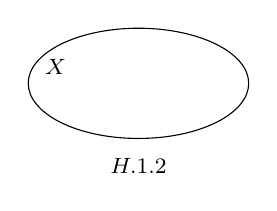
\begin{tikzpicture}[>=stealth,line join=round,line cap=round,font=\footnotesize,scale=.7]
			\draw (1,1) circle (2 and 1);
			\coordinate[label=center:$X$] (X)at(-.5,1.3);
			\coordinate[label=center:$ H.1.2$] (X)at(1,-.5);
	\end{tikzpicture}}
	\immini {$\bullet$ Minh hoạ $T$ là một tập con của $S$ như Hình $1.3$.}
	{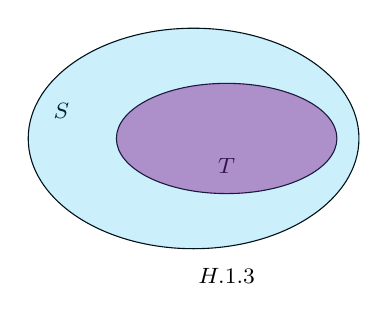
\begin{tikzpicture}[>=stealth,line join=round,line cap=round,font=\footnotesize,scale=.7]
			\coordinate[label=center:$$] (I)at(.4,1);
			\coordinate[label=center:$$] (M)at(1,1);
			\draw (.4,1) circle (3 and 2);
			\coordinate[label=center:$S$] (X)at(-2,1.5);
			\draw (1,1) circle (2 and 1);
			\coordinate[label=center:$T$] (X)at(1,.5);
			\coordinate[label=center:$ H.1.3$] (X)at(1,-1.5);
			\fill[cyan,opacity=.2] (I) ellipse (3 cm and 2 cm)--cycle;
			\fill[violet,opacity=.4] (M) ellipse (2 cm and 1 cm)--cycle;
	\end{tikzpicture}}
\end{tcolorbox}
\subsubsection{Hai tập hợp bằng nhau}
\begin{tcolorbox}
	$S=T \Leftrightarrow \heva{& S \subset T \\ & T \subset S} \Leftrightarrow \forall x,\ (x\in S \Leftrightarrow x \in T)$
\end{tcolorbox}

\subsubsection{Mối quan hệ giữa các tập hợp số}
$\bullet$ Tập hợp các số tự nhiên $\mathbb{N}=\{0 ; 1 ; 2 ; 3 ; \ldots\}$.\\
$\bullet$ Tập hợp các số nguyên $\mathbb{Z}$ gồm các số tự nhiên và các số nguyên âm:
$\mathbb{Z}=\{\ldots ;-2 ;-1 ; 0 ; 1 ; 2 ; \ldots\}$.
$\bullet$ Tập hợp các số hữu tỉ $\mathbb{Q}$ gồm các số viết được dưới dạng phân số $\dfrac{a}{b}$, với $a, b \in \mathbb{Z}, b \neq 0$. Số hữu tỉ còn được biểu diễn dưới dạng số thập phân hữu hạn hoặc vô hạn tuần hoàn.\\
$\bullet$ Tập hợp các số thực $\mathbb{R}$ gồm các số hữu tỉ và các số vô tỉ. Số vô tỉ là các số thập phân vô hạn không tuần hoàn.
\begin{tcolorbox}
	\immini { Mối quan hệ giữa các tập hợp số:  $\mathbb{N} \subset \mathbb{Z} \subset \mathbb{Q} \subset \mathbb{R}$.}
	{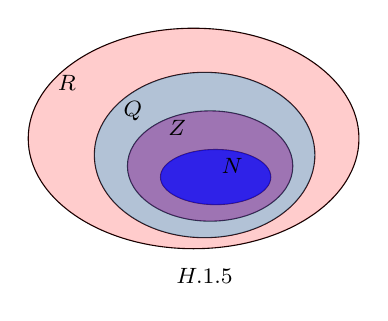
\begin{tikzpicture}[>=stealth,line join=round,line cap=round,font=\footnotesize,scale=.7]
			\path (1.3,1)coordinate[label=center:$$](M) (1.5,.7)coordinate[label=center:$$](N) (1.6,.5)coordinate[label=center:$$](P) (1.7,.3)coordinate[label=center:$$](Q)
			(1.5,-1.5)coordinate[label=center:$H.1.5$](H);
			\draw (1.3,1) circle (3 and 2);
			\draw (1.5,.7) circle (2 and 1.5);
			\draw (1.6,.5) circle (1.5 and 1);
			\draw (1.7,.3) circle (1 and .5);
			\fill[red,opacity=.2] (M) ellipse (3 cm and 2 cm)--cycle;
			\fill[cyan,opacity=.3] (N) ellipse (2 cm and 1.5 cm)--cycle;
			\fill[violet,opacity=.4] (P) ellipse (1.5 cm and 1 cm)--cycle;
			\fill[blue,opacity=.7] (Q) ellipse (1 cm and .5 cm)--cycle;
			\coordinate[label=center:$\mathbb{R}$] (X)at(-1,2);
			\coordinate[label=center:$\mathbb{Q}$] (Q)at(0.2,1.5);
			\coordinate[label=center:$\mathbb{Z}$] (Z)at(1,1.2);
			\coordinate[label=center:$\mathbb{N}$] (N)at(2,.5);
	\end{tikzpicture}}
\end{tcolorbox}
\subsubsection{Các tập con thường dùng của $\mathbb{R}$}
\begin{tcolorbox}
	Một số tập con thường dùng của tập số thực $\mathbb{R}$.\\
	$\bullet$ Khoảng\\
	\immini {$(a ; b)=\{x \in \mathbb{R} \mid a<x<b\}$} {\begin{tikzpicture}[>=stealth,line join=round,line cap=round,font=\footnotesize,scale=1]
			\draw[->] (0,0)--(6,0);
			\path[pattern=north east lines,pattern color=blue] (0,-3pt)rectangle(2,3pt);
			\path[pattern=north east lines,pattern color=blue] (6,-3pt)rectangle(4,3pt);
			\path 
			(2,-0.1)coordinate[label=below:$a$](a) 
			(4,-0.1)coordinate[label=below:$b$](b)
			(2,0)coordinate[label=center:$($](()
			(4,0)coordinate[label=center:$)$](s);
	\end{tikzpicture}}
	\immini {$(a ;+\infty)=\{x \in \mathbb{R} \mid x>a\}$}
	{\begin{tikzpicture}[>=stealth,line join=round,line cap=round,font=\footnotesize,scale=1]
			\draw[->] (0,0)--(6,0);
			\path[pattern=north east lines,pattern color=blue] (0,-3pt)rectangle(2,3pt);
			%\path[pattern=north east lines,pattern color=blue] (6,-3pt)rectangle(4,3pt);
			\path 
			(2,-0.1)coordinate[label=below:$a$](a) 
			%(4,0)coordinate[label=below:$a$](b)
			(2,0)coordinate[label=center:$($](()
			%(4,0)coordinate[label=center:$)$](s)
			;
	\end{tikzpicture}}
	\immini {$(-\infty ; b)=\left\{x \in \mathbb{R} \mid x<b\right\}$}
	{\begin{tikzpicture}[>=stealth,line join=round,line cap=round,font=\footnotesize,scale=1]
			\draw[->] (0,0)--(6,0);
			%\path[pattern=north east lines,pattern color=blue] (0,-3pt)rectangle(2,3pt);
			\path[pattern=north east lines,pattern color=blue] (6,-3pt)rectangle(4,3pt);
			\path 
			%(2,0)coordinate[label=below:$a$](a) 
			(4,-0.1)coordinate[label=below:$b$](b)
			%(2,0)coordinate[label=center:$($](()
			(4,0)coordinate[label=center:$)$](s)
			;
	\end{tikzpicture}}
	\immini {$(-\infty ;+\infty)$}
	{\begin{tikzpicture}[>=stealth,line join=round,line cap=round,font=\footnotesize,scale=1]
			\draw[->] (0,0)--(6,0);
			%\path[pattern=north east lines,pattern color=blue] (0,-3pt)rectangle(2,3pt);
			%\path[pattern=north east lines,pattern color=blue] (6,-3pt)rectangle(4,3pt);
			\path 
			(3,-0.1)coordinate[label=below:$O$](a) 
			%(4,0)coordinate[label=below:$a$](b)
			(3,0)coordinate[label=center:$|$](()
			%(4,0)coordinate[label=center:$)$](s)
			;
	\end{tikzpicture}}
	$\bullet$ Đoạn\\
	\immini {$[a ; b]=\{x \in \mathbb{R} \mid a \leq x \leq b\}$}
	{\begin{tikzpicture}[>=stealth,line join=round,line cap=round,font=\footnotesize,scale=1]
			\draw[->] (0,0)--(6,0);
			\path[pattern=north east lines,pattern color=blue] (0,-3pt)rectangle(2,3pt);
			\path[pattern=north east lines,pattern color=blue] (6,-3pt)rectangle(4,3pt);
			\path 
			(2,-0.1)coordinate[label=below:$a$](a) 
			(4,-0.1)coordinate[label=below:$b$](b)
			(2,0)coordinate[label=center:$[$]()
			(4,0)coordinate[label=center:$\mathrm{]}$](s);
	\end{tikzpicture}}
	$\bullet$ Nửa khoảng\\
	\immini {$[a ; b)=\{x \in \mathbb{R} \mid a \leq x<b\}$}
	{\begin{tikzpicture}[>=stealth,line join=round,line cap=round,font=\footnotesize,scale=1]
			\draw[->] (0,0)--(6,0);
			\path[pattern=north east lines,pattern color=blue] (0,-3pt)rectangle(2,3pt);
			\path[pattern=north east lines,pattern color=blue] (6,-3pt)rectangle(4,3pt);
			\path 
			(2,-0.1)coordinate[label=below:$a$](a) 
			(4,-0.1)coordinate[label=below:$b$](b)
			(2,0)coordinate[label=center:$[$]()
			(4,0)coordinate[label=center:$\mathrm{)}$](s);
	\end{tikzpicture}}
	\immini {$(a ; b]=\{x \in \mathbb{R} \mid a<x \leq b\}$}
	{\begin{tikzpicture}[>=stealth,line join=round,line cap=round,font=\footnotesize,scale=1]
			\draw[->] (0,0)--(6,0);
			\path[pattern=north east lines,pattern color=blue] (0,-3pt)rectangle(2,3pt);
			\path[pattern=north east lines,pattern color=blue] (6,-3pt)rectangle(4,3pt);
			\path 
			(2,-0.1)coordinate[label=below:$a$](a) 
			(4,-0.1)coordinate[label=below:$b$](b)
			(2,0)coordinate[label=center:$($]()
			(4,0)coordinate[label=center:$\mathrm{]}$](s);
	\end{tikzpicture}}
	\immini {$[a ;+\infty)=\{x \in \mathbb{R} \mid x \geq a\}$}
	{\begin{tikzpicture}[>=stealth,line join=round,line cap=round,font=\footnotesize,scale=1]
			\draw[->] (0,0)--(6,0);
			\path[pattern=north east lines,pattern color=blue] (0,-3pt)rectangle(2,3pt);
			%\path[pattern=north east lines,pattern color=blue] (6,-3pt)rectangle(4,3pt);
			\path 
			(2,-0.1)coordinate[label=below:$a$](a) 
			%(4,0)coordinate[label=below:$a$](b)
			(2,0)coordinate[label=center:$[$](()
			%(4,0)coordinate[label=center:$)$](s)
			;
	\end{tikzpicture}}
	\immini {$(-\infty ; b]=\{x \in \mathbb{R} \mid x \leq b\}$}
	{\begin{tikzpicture}[>=stealth,line join=round,line cap=round,font=\footnotesize,scale=1]
			\draw[->] (0,0)--(6,0);
			%\path[pattern=north east lines,pattern color=blue] (0,-3pt)rectangle(2,3pt);
			\path[pattern=north east lines,pattern color=blue] (6,-3pt)rectangle(4,3pt);
			\path 
			%(2,0)coordinate[label=below:$a$](a) 
			(4,-0.1)coordinate[label=below:$b$](b)
			%(2,0)coordinate[label=center:$($](()
			(4,0)coordinate[label=center:$\mathrm{]}$](s)
			;
	\end{tikzpicture}}
\end{tcolorbox}

\subsubsection{Giao của hai tập hợp}
\begin{tcolorbox}
	\immini{Tập hợp gồm các phần tử thuộc cả hai tập hợp $S$ và $T$ gọi là giao của hai tập hợp $S$ và $T$, kí hiệu là $S \cap T$.\\
		$S \cap T=\{x \mid x \in S$ và $x \in T\}$.}
	{\begin{tikzpicture}[>=stealth,line join=round,line cap=round,font=\footnotesize,scale=1]
			\begin{scope}
				\clip (0.5,0) ellipse (1.5 and 1 );
				\fill[pattern = north east lines]	(2.5,0) ellipse (2 and 1.5 );
			\end{scope}
			\draw (0.5,0) ellipse (1.5 and 1 );
			\draw (2.5,0) ellipse (2 and 1.5 );
			\coordinate[label=center:$S\cap T$] (M)at(1.1,.3);
	\end{tikzpicture}}
\end{tcolorbox}
\subsubsection{Hợp của hai tập hợp}
\begin{tcolorbox}
	\immini {Tập hợp gồm các phần tử thuộc tập hợp $S$ hoặc thuộc tập hợp $T$ gọi là hợp của hai tập hợp $S$ và $T$. Kí hiệu là $S \cup T$.
		\[S \cup T=\{x \mid x \in S \text { hoặc } x \in T\}.\]}
	{\begin{tikzpicture}[>=stealth,line join=round,line cap=round,font=\footnotesize,scale=.7]
			\coordinate[label=center:$$] (I)at(0,1);
			\coordinate[label=center:$$] (M)at(1,1);
			\draw[fill,pattern = north east lines] (0,1) circle (1.5 and 1);
			\draw[fill,pattern = north east lines] (1,1) circle (1.5 and 1);
			\coordinate[label=center:$S\cup T$] (X)at(.6,-.5);
			\coordinate[label=center:$S$] (X)at(-1,1);
			\coordinate[label=center:$T$] (X)at(2,1);
	\end{tikzpicture}}
\end{tcolorbox}
\subsubsection{Hiệu của hai tập hợp}
\begin{tcolorbox}
	\immini {$\bullet$ Hiệu của hai tập hợp $S$ và $T$ là tập hợp gồm các phần tử thuộc S nhưng không thuộc $T$, kí hiệu là $S \backslash T$.
		\[S \backslash T=\{x \mid x \in S \text{ và } x \notin T\}\].}
	{\begin{tikzpicture}[>=stealth,line join=round,line cap=round,font=\footnotesize,scale=.8]
			\draw (0.5,0) ellipse (1.5 and 1 );
			\draw (2.5,0) ellipse (1.5 and 1 );
			\fill[pattern = north east lines] (0.5,0) ellipse (1.5 and 1 );
			\fill[fill=white] (2.5,0) ellipse (1.5 and 1 );
			\path 
			(0,.5)coordinate[label=center:$S$](S) (2,.5)coordinate[label=center:$T$](T)
			(1.7,1.5)coordinate[label=center:$S\backslash T$](T) ;
			
	\end{tikzpicture}}
	\immini {$\bullet$ Nếu $T \subset S$ thì $S \backslash T$ được gọi là phần bù của $T$ trong $S$, kí hiệu là $C_{s} T$.}
	{	\begin{tikzpicture}[>=stealth,line join=round,line cap=round,font=\footnotesize,scale=.8]
			\draw (0.5,0) ellipse (1.5 and 1 );
			\draw (.8,0) ellipse (1 and .5 );
			\fill[pattern = north east lines] (0.5,0) ellipse (1.5 and 1 );
			\fill[fill=white] (.8,0) ellipse (1 and .5 );
			\path 
			(-.3,.5)coordinate[label=center:$S$](S) (1,0)coordinate[label=center:$T$](T)
			(1,1.3)coordinate[label=center:$C_S T$](T) ;
			
	\end{tikzpicture}}
\end{tcolorbox}
\subsection{CÁC DẠNG BÀI TẬP}
\begin{dang}{Xác định tập hợp}
	Được mô tả theo 2 cách:
	\begin{enumEX}{1}
		\item  Liệt kê tất cả các phần tử của tập hợp.
		\item  Nêu tính chất đặc trưng.
	\end{enumEX}
\end{dang}
\subsubsection{Ví dụ minh hoạ}
\begin{vd}%[BG10-2022]%[Đỗ Văn Dự]%[0D1Y2-1]
	Cho $D=\{n \in \mathbb{N} \mid n$ là số nguyên tố, $5<n<20\}$.
	\begin{enumEX}{1}
		\item Dùng kí hiệu $\in, \notin$ để viết câu trả lời cho câu hỏi sau: Trong các số $5$; $12$; $17$; $18$, số nào thuộc tập $D$, số nào không thuộc tập $D$?
		\item Viết tập hợp $D$ bằng cách liệt kê các phần tử. Tập hợp $D$ có bao nhiêu phần tử?
	\end{enumEX}
	\loigiai{
		\begin{enumEX}{1}
			\item $5 \notin D$; $12 \notin D$; $17 \in D$; $18 \notin D$.
			\item $D=\{7 ; 11 ; 13 ; 17 ; 19\}$. Tập hợp $D$ có $5$ phần tử.
		\end{enumEX}	
	}
\end{vd}

\begin{vd}%[BG10-2022]%[Đỗ Văn Dự]%[0D1B2-1] 
	Viết mỗi tập hợp sau bằng cách liệt kê các phần tử.
	\begin{enumEX}{2}
		\item $A=\left\{\left. x\in \mathbb{R}\right|\left(2x-x^2\right)\left(3x-2\right)=0\right\}$.
		\item $B=\left\{\left. x\in \mathbb{Z}\right|2x^3-3x^2-5x=0\right\}$.
		\item $C=\left\{\left. x\in \mathbb{Z}\right|2x^2-75x-77=0\right\}$.
		\item $D=\left\{\left. x\in \mathbb{R}\right|(x^2-x-2)(x^2-9)=0\right\}$.
	\end{enumEX}
	\loigiai{
		\begin{enumEX}{1}
			\item Ta giải phương trình\\
			 $\left(2x-x^2\right)\left(2x^2-3x-2\right)=0\Leftrightarrow \hoac{
				& 2x-x^2=0 \\ 
				& 2x^2-3x-2=0}\Leftrightarrow \hoac{
				& x=0\vee x=2 \\ 
				& x=-\dfrac{1}{2}\vee x=2}$.\\
			Do $x\in \mathbb{R}$ nên $A=\left\{-\dfrac{1}{2};0;2\right\}$.
			\item Ta giải phương trình $2x^3-3x^2-5x=0\Leftrightarrow x\left(2x^2-3x-5\right)=0\Leftrightarrow \hoac{&x=0\\&x=-1\\&x=\dfrac{5}{3}}$.\\
			Do $x\in \mathbb{Z}$ nên $B=\left\{0;-1\right\}$.
			\item Ta giải phương trình $2x^2-75x-77=0\Leftrightarrow \hoac{&x=-1\\&x=\dfrac{77}{2}}$.\\
			Do $x\in \mathbb{Z}$ nên $C=\left\{-1\right\}$.
	\end{enumEX}}
\end{vd}

\begin{vd}%[BG10-2022]%[Đỗ Văn Dự]%[0D1B2-1] 
	Viết mỗi tập hợp sau bằng cách liệt kê các phần tử.
	\begin{enumEX}{1}
		\item $A=\left\{\left. n\in {\mathbb{N}}^{*}\right|3<n^2<30\right\}$.
		\item $B=\left\{\left. n\in \mathbb{Z}\right|\left| n\right|<3\right\}$.
		\item $C=\left\{\left. x\right|x=3k\right.$ với $k\in \mathbb{Z}$ và $\left.-4<x<12\right\}$.
		\item $D=\left\{\left. n^2+3\right|n \in \mathbb{N} \text{ và } n<5\right\}$.
	\end{enumEX}
	\loigiai{
		\begin{enumEX}{1}
			\item Với $3<n^2<30$ và $n\in {\mathbb{N}}^{*}$ nên chọn $n=2;3;4;5$.\\
			Vậy $A=\left\{2;3;4;5\right\}$.
			\item  Vì $x<\left| 3\right|\Leftrightarrow-3<x<3$.\\
			Do $x\in \mathbb{Z}$ nên $B=\left\{-2;-1;0;1;2\right\}$.
			\item Ta có $-4<x<12\Leftrightarrow-4<3k<12\Leftrightarrow-\dfrac{4}{3}<k<4$.\\
			Do $k\in \mathbb{Z}$ nên ta chọn $k=\left\{-10;1;2;3\right\}$ suy ra $x=3k=\left\{-3;0;3;6;9\right\}$.\\
			Vậy $C=\left\{-3;0;3;6;9\right\}$.
			\item Vì $n \in \mathbb{N} \text{ và } n<5$ nên chọn  $n=0,1,2;3;4$.\\
			Vậy $A=\left\{3;4;12;19\right\}$.
		\end{enumEX}
	}
\end{vd}

\begin{vd}%[BG10-2022]%[Đỗ Văn Dự]%[0D1K2-1]
	Viết mỗi tập hợp sau bằng cách nêu tính chất đặc trưng.
	\begin{enumEX}{2}
		\item $A=\left\{\dfrac{2}{3};\dfrac{3}{8};\dfrac{4}{15};\dfrac{5}{24};\dfrac{6}{35}\right\}$.
		\item $B=\left\{0;3;8;15;24;35\right\}$.
		\item $C=\left\{-4;1;6;11;16\right\}$.
		\item $D=\left\{1;-2;7\right\}$.
	\end{enumEX}
	\loigiai{
		\begin{enumEX}{2}
			\item $A=\left\{\left. \dfrac{n}{n^2-1}\right|n\in \mathbb{N},2\le n\le 6\right\}$.
			\item $B=\left\{\left. n^2-1\right|n\in \mathbb{N},1\le n\le 6\right\}$.
			\item $C=\left\{\left. n\in \mathbb{N}\right|\right.\left. 5n-4\right\}$.
			\item $D=\left\{\left. x\in \mathbb{R}\right|\left(x-1\right)\left(x+2\right)\left(x-7\right)=0\right\}$.
		\end{enumEX}
	}
\end{vd}
\subsubsection{Bài tập tự luận}
\begin{bt}%[Huỳnh Quy]%[0D1B2-1]
	Liệt kê các phần tử của các tập hợp sau:
	\begin{enumerate}
		\item $A=\left\lbrace n\in \mathbb{N} \mid n<5\right\rbrace$.
		\item $B$ là tập hợp các số tự nhiên lớn hơn $0$ và nhỏ hơn $5$.
		\item $C=\left\lbrace x\in \mathbb{R}\mid (x-1)(x+2)=0\right\rbrace$.
	\end{enumerate}
	\loigiai{
		\begin{enumerate}
			\item $A=\left\lbrace 0;1;2;3;4\right\rbrace$.
			\item $B=\left\lbrace 1;2;3;4\right\rbrace$.
			\item Ta có $(x-1)(x+2)=0 \Leftrightarrow \hoac{&x=1\\&x=-2.}$\\
			Mà $x\in \mathbb{R}$ nên
			$C=\left\lbrace -2;1\right\rbrace$.
		\end{enumerate}
	}
\end{bt}
\begin{bt}%[Huỳnh Quy]%[0D1B2-1]
	Viết các tập hợp sau bằng phương pháp liệt kê:
	\begin{enumerate}
		\item $A=\left\lbrace  x\in \mathbb{Q}\mid (x^2-2x+1)(x^2-5)\right\rbrace=0$.
		\item $B=\left\lbrace x \in \mathbb{N}\mid 5<x^2<40\right\rbrace$.
		\item $C=\left\lbrace x\in \mathbb{Z}\mid x^2<9\right\rbrace$.
		\item $D=\left\lbrace x\in \mathbb{R}\mid \left|2x+1\right|=5\right\rbrace$.
	\end{enumerate}
	\loigiai{
		\begin{enumerate}
			\item Ta có $x\in A\Leftrightarrow\hoac{&x^2-2x+1=0\\&x^2-5=0}\Leftrightarrow\hoac{&x=1\in\mathbb{Q}\\&x=\pm\sqrt{5}\not\in \mathbb{Q}.}$\\
			Vậy $A=\left\lbrace 1\right\rbrace$.
			\item $B=\left\lbrace 3;4;5;6\right\rbrace$.
			\item $C=\left\lbrace -2;-1;0;1;2\right\rbrace$.
			\item Ta có $\left|2x+1\right|=5\Leftrightarrow \hoac{& 2x+1=5 \\ & 2x+1 =-5} \Leftrightarrow \hoac{&x=2\\&x=-3.}$\\
			Vậy $D=\left\lbrace 2;-3\right\rbrace$.
		\end{enumerate}
	}
\end{bt}
\begin{bt}%[Huỳnh Quy]%[0D1B2-1]
	Viết các tập hợp sau bằng cách chỉ ra tính chất đặc trưng cho các phần tử của tập hợp đó.
	\begin{enumerate}
		\item $A=\left\lbrace 0;4;8;12;16;\ldots ;52\right\rbrace$.
		\item $B=\left\lbrace 3;6;9;12;15;\ldots ;51\right\rbrace$.
		\item $C=\left\lbrace 2;5;8;11;14;\ldots ;62\right\rbrace$.
	\end{enumerate}
	\loigiai{
		\begin{enumerate}
			\item $A=\left\lbrace x\in \mathbb{N}\mid 0\le x\le 52 \text{ và } x\;\vdots \;4\right\rbrace$.
			\item $B=\left\lbrace x\in \mathbb{N}\mid 3\le x\le 51 \text{ và } x\;\vdots \;3\right\rbrace$.
			\item $C=\left\lbrace  x\in \mathbb{N}\mid 2\le x\le 62 \text{ và } (x-2)\;\vdots \;3\right\rbrace$.
		\end{enumerate}
	}
\end{bt}
\begin{bt}%[Huỳnh Quy]%[0D1K2-1]
	Viết các tập hợp sau bằng cách chỉ ra tính chất đặc trưng cho các phần tử của tập hợp đó.
	\begin{enumerate}
		\item $A=\left\lbrace 2;3;5;7;11;13;17\right\rbrace$.
		\item $B=\left\lbrace -2;4;-8;16;-32;64\right\rbrace$.
	\end{enumerate}
	\loigiai{
		\begin{enumerate}
			\item $A=\left\lbrace x\in \mathbb{N}\mid x\le 17 \text{ và }x \text{ là số nguyên tố} \right\rbrace$.
			\item $B=\left\lbrace x=(-2)^n\mid n\in \mathbb{N}, 1\le n\le 6 \right\rbrace$.
		\end{enumerate}
	}
\end{bt}

\begin{bt}%[Huỳnh Quy]%[0D1B2-1]
	Tìm một tính chất đặc trưng xác định các phần tử của mỗi tập hợp sau
	\begin{align*}
		A&=\{1; 2; 3; 4; 5; 6; 7; 8; 9\} \\
		B&=\{0; 7; 14; 21; 28\}
	\end{align*}
	\loigiai{
		\begin{align*}
			A&=\{x\in \mathbb{N^*} \mid x\leq 9\} \\
			B&=\{x\in \mathbb{N} \mid x \;\vdots \;7 \text{ và } x\leq 28\}
		\end{align*}
	}
\end{bt}

\begin{dang}{Tập hợp con, xác định tập hợp con}
	Cho tập hợp $A$ gồm $n$ phần tử.
	\begin{enumEX}{1}
		\item  Khi liệt kê tất cả các tập con của $A$, ta liệt kê đầy đủ theo thứ tự:\\		
		\centerline{ $\varnothing$; tập $1$ phần tử; tập $2$ phần tử; tập $3$ phần tử;...; $A$.}
		\item  Số tập con của $A$ là $2^n$.
		\item  Số tập con gồm $k$ phần tử của $A$ là $\mathrm{C}_n^k$.
	\end{enumEX}
\end{dang}
\subsubsection{Ví dụ minh hoạ}
\begin{vd}%[BG10-2022]%[Đỗ Văn Dự]%[0D1Y2-2]
	Cho tập hợp $S=\{2 ; 3 ; 5\}$. Những tập hợp nào sau đây là tập con của $S$?
	$$S_{1}=\{3\};S_{2}=\{0 ; 2\}; S_{3}=\{3 ; 5\}$$.
	\loigiai{
		Các tập hợp $S_{1}=\{3\}$, $S_{3}=\{3 ; 5\}$ là những tập con của $S$.\\
		Tập $S_{2}=\{0 ; 2\}$ không là tập con của $S$.
	}
\end{vd}

\begin{vd}%[BG10-2022]%[Đỗ Văn Dự]%[0D1B2-2]
	Cho tập hợp $A=\left\{2;3;4\right\}$ và $B=\left\{2;3;4;5;6\right\}$.
	\begin{enumEX}{1}
		\item Xác định tất cả tập con có hai phần tử của $A$.
		\item Xác định tất cả tập con có ít hơn hai phần tử của $A$.
		\item Tập $A$ có tất cả bao nhiêu tập con.
		\item Xác định tất cả các tập $X$ thỏa $A \subset X \subset B$.
	\end{enumEX}
		\loigiai{
	\begin{enumEX}{1}		
		\item 	Các tập hợp $S_1=\{2;3\}$, $S_2=\{2;4\}$, $S_3=\{3;4\}$  là những tập con của $A$.\\
			Tập $S_{2}=\{0 ; 2\}$ không là tập con của $S$.
		\item 	Các tập hợp $\varnothing$, $\{2\}$, $\{3\}$, $\{4\}$  là những tập con ít hơn $2$ phần tử của $A$.\\
		\item 	Tập $A$ có tất cả $8$ tập con.
		\item 	 Tất cả các tập $X$ thỏa $A \subset X \subset B$ là $\{2;3;4\}$, $\{2;3;4,5\}$, $\{2;3;4,5,6\}$.	
	\end{enumEX}
		}	
\end{vd}
\subsubsection{Bài tập tự luận}
\begin{bt}%[Huỳnh Quy]%[0D1B2-2]
	Tìm tất cả các tập con của tập $A=\{a,1,2\}$.
	\loigiai{Tập $A$ có $2^3=8$ tập con.
		\begin{itemize}
			\item 0 phần tử: $ \varnothing $.
			\item 1 phần tử: $\{a\}$, $\{1\}$, $\{2\}$.
			\item 2 phần tử: $\{a, 1\}$, $\{a,2\}$, $\{1,2\}$.
			\item 3 phần tử: $\{a,1,2\}$.
	\end{itemize}}
\end{bt}
\begin{bt}%[Huỳnh Quy]%[0D1B2-2]
	Tìm tất cả các tập con có 2 phần tử của tập $A=\{1,2,3,4,5,6\}$.
	\loigiai{$\{1,2\}$,$\{1,3\}$, $\{1,4\}$, $\{1,5\}$, $\{1,6\}$, $\{2,3\}$, $\{2,4\}$, $\{2,5\}$, $\{2,6\}$, $\{3,4\}$, $\{3,5\}$, $\{3,6\}$, $\{4,5\}$, $\{4,6\}$, $\{5,6\}$.}
\end{bt}
\begin{bt}%[Huỳnh Quy]%[0D1B2-2]
	Xác định tập hợp $X$ biết $\{1,2\} \subset X \subset \{1,2,5\}$.
	\loigiai{Ta có
		\begin{itemize}
			\item  Vì $\{1,2\} \subset X$ nên tập hợp $X$ có chứa các phần tử $1,2$.
			\item  Vì $X \subset \{1,2,5\}$ nên các phần tử của tập hợp $X$ có thể là $1,2,5$.
		\end{itemize}
		Khi đó tập hợp $X$ có thể là $\{1,2\}, \{1,2,5\}$.}
\end{bt}
\begin{bt}%[Huỳnh Quy]%[0D1B2-2]
	Xác định tập hợp $X$ biết $\{a,1\} \subset X \subset \{a,b,1,2\}$.
	\loigiai{Ta có
		\begin{itemize}
			\item  Vì $\{a,1\} \subset X$ nên tập hợp $X$ có chứa 2 phần tử là $a,1$.
			\item  Vì $X \subset \{a,b,1,2\}$ nên các phần tử của tập hợp $X$ có thể là $a,b,1,2$.
		\end{itemize}
		Suy ra, tập hợp $X$ có 2 phần tử, 3 phần tử hoặc 4 phần tử.\\
		Khi đó, tập hợp $X$ có thể là $\{a,1\}, \{a,1,2\}, \{a,b,1\}, \{a,b,2\}, \{a,b,1,2\}$.\\
		\underline{\textbf{Cách khác:}} $X=\{a;1\} \cup X'$ với $X' \subset \{b;2\}$. \\
		Vì có $4$ tập hợp $X'$ nên có $4$ tập hợp $X$ thỏa yêu cầu bài toán.}
\end{bt}
\begin{bt}%[Huỳnh Quy]%[0D1K2-2]
	Cho tập hợp $A=\{1;2;3;4;5;6\}$. Tìm tất cả các tập con có $3$ phần tử của tập hợp $A$ sao cho tổng các phần tử này là một số lẻ.
	\loigiai{
		Để tổng của ba số nguyên là một số lẻ thì trong ba số chỉ có một số lẻ hoặc cả ba số đều lẻ. Nói cách khác tập con này của $A$ phải có một số lẻ hoặc ba số lẻ.\\
		Chỉ có một tập con gồm ba số lẻ của $A$ là $\{1;3;5\}$. Các tập con gồm ba số của $A$ trong đó có một số lẻ là: \\
		$\{1;2;4\}$; $\{1;2;6\}$; $\{1;4;6\}$;$\{3;2;4\}$; $\{3;2;6\}$; $\{3;4;6\}$; $\{5;2;4\}$; $\{5;2;6\}$; $\{5;4;6\}$.\\
		\textit{\underline{Nhận xét:} Tổng các số nguyên là một số lẻ khi số số lẻ là số lẻ.}
	}
\end{bt}
\begin{bt}%[Huỳnh Quy]%[0D1K2-2]
	Cho $A=\{n\in\mathbb{N}\mid n \text{ là ước của }2\}$; $B=\{x\in\mathbb{R}\mid (x^2-1)(x-2)(x-4)=0 \}$. Tìm tất cả các tập hợp $X$ sao cho $A\subset X\subset B$.
	\loigiai{ 
		Liệt kê các phần tử của tập hợp $A$ và $B$ ta được : \\
		$A=\{1;2\}$; $B=\{-1;1;2;4\}$.\\
		Muốn tìm tập $X$ thỏa điều kiện $A\subset X\subset B$ đầu tiên ta lấy $X=A$, sau đó ghép thêm các phần tử thuộc $B$ mà không thuộc $A$. Với cách thực hiện như trên, ta có các tập hợp $X$ thỏa mãn yêu cầu bài toán là: $X=A=\{1;2 \}$, rồi ghép thêm vào một phần tử ta được: $\{-1;1;2 \}$;$\{4;1;2 \}$\\
		Ghép thêm vào $A$ hai trong bốn phần tử còn lại của $B$ ta được : $X=B=\{-1;1;2;4\}$
	}
\end{bt}
\begin{dang}{Các phép toán trên tập hợp}
\end{dang}
\subsubsection{Ví dụ minh hoạ}
\begin{vd}%[BG10-2022]%[Đỗ Văn Dự]%[0D1B2-2]
	Cho hai tập hợp:
	$C=\{n \in \mathbb{N} \mid n$ là bội chung của 2 và $3 ; n<30\}$;
	$D=\{n \in \mathbb{N} \mid n$ là bội của $6 ; n<30\}$.
	Chứng minh rằng $C=D$.
	\loigiai{
		Ta có: $C=\{0 ; 6 ; 12 ; 18 ; 24\}$.\\
		$D=\{0 ; 6 ; 12 ; 18 ; 24\}$.\\
		Vậy $C=D$.
	}
\end{vd}

\begin{vd}%[BG10-2022]%[Đỗ Văn Dự]%[0D1Y4-1]
	Viết các tập hợp sau dưới dạng các khoảng, đoạn, nửa khoảng trong $\mathbb{R}$ rồi biểu diễn trên trục số: $C=\{x \in \mathbb{R} \mid 2 \leq x \leq 7\}$; $D=\{x \in \mathbb{R} \mid x<2\}$.
	\loigiai{
		\immini{$C=[2;7]$}{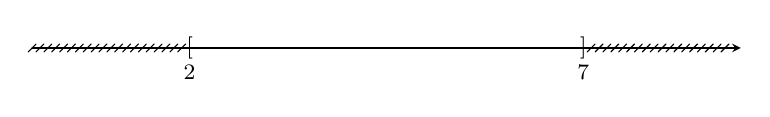
\begin{tikzpicture}[scale=1,>=stealth, font=\footnotesize, line join=round, line cap=round]
				\draw [-stealth] (0,0)--(9,0);
				\path (2,0) node{$[$} (2,-0.1)node[below]{$2$}
				(7,0) node{$]$} (7,-0.1)node[below]{$7$};
				\foreach \x in{0,0.1,...,2} \draw (\x,0)--++(45:.07) (\x,0)--++(-135:.07);
				\foreach \x in{7.1,7.2,...,8.8} \draw (\x,0)--++(45:.07) (\x,0)--++(-135:.07);
		\end{tikzpicture}}
		\immini{$C=(-\infty;2)$}{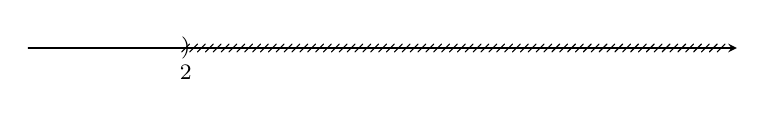
\begin{tikzpicture}[scale=1,>=stealth, font=\footnotesize, line join=round, line cap=round]
				\draw [-stealth] (0,0)--(9,0);
				\path (2,0) node{$)$} (2,-0.1)node[below]{$2$};
				\foreach \x in{2,2.1,...,8.9} \draw (\x,0)--++(45:.07) (\x,0)--++(-135:.07);
		\end{tikzpicture}}	
		
	}
\end{vd}

\begin{vd}%[BG10-2022]%[Đỗ Văn Dự]%[0D1B4-1]
	\begin{enumerate}
		\item Cho hai tập hợp $C=\{4 ; 7 ; 27\}$ và $D=\{2 ; 4 ; 9 ; 27 ; 36\}$. Hãy xác định tập hợp $C \cap D$.
		\item Cho hai tập hợp $E=[1 ;+\infty)$ và $F=(-\infty ; 3]$. Hãy xác định tập hợp $E \cap F$.
	\end{enumerate}
	\loigiai{
		\begin{enumEX}{1}
			\item Giao của hai tập hợp $C$ và $D$ là $C \cap D=\{4 ; 27\}$.
			\item Giao của hai tập hợp $E$ và $F$ là $E \cap F=[1 ; 3]$.\\
			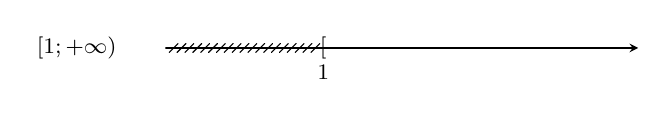
\begin{tikzpicture}[scale=1,>=stealth, font=\footnotesize, line join=round, line cap=round]
				\draw [-stealth] (-1,0)--(5,0);
				\path (1,0) node{$[$} (1,-0.1)node[below]{$1$} (-1.5,0)node[left]{$[1 ;+\infty)$};
				\foreach \x in{-0.9,-0.8,...,0.9} \draw (\x,0)--++(45:.08) (\x,0)--++(-135:.08);
			\end{tikzpicture}\\
			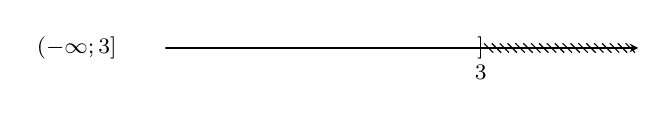
\begin{tikzpicture}[scale=1,>=stealth, font=\footnotesize, line join=round, line cap=round]
				\draw [-stealth] (-1,0)--(5,0);
				\path (3,0) node{$]$} (3,-0.1)node[below]{$3$} (-1.5,0)node[left]{$(-\infty ; 3]$};
				\foreach \x in{3.1,3.2,...,4.9} \draw (\x,0)--++(-45:.08) (\x,0)--++(135:.08);
			\end{tikzpicture}\\
			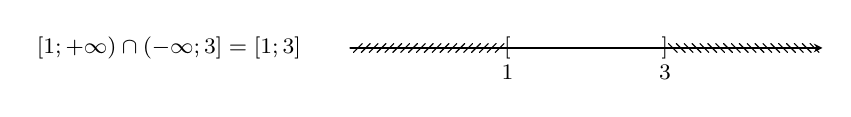
\begin{tikzpicture}[scale=1,>=stealth, font=\footnotesize, line join=round, line cap=round]
				\draw [-stealth] (-1,0)--(5,0);
				\path (3,0) node{$]$} (3,-0.1)node[below]{$3$} 
				(1,0) node{$[$} (1,-0.1)node[below]{$1$} (-1.5,0)node[left]{$[1 ;+\infty)\cap(-\infty ; 3]=[1;3]$}
				;
				\foreach \x in{3.1,3.2,...,4.9} \draw (\x,0)--++(-45:.08) (\x,0)--++(135:.08);
				\foreach \x in{-0.9,-0.8,...,0.9} \draw (\x,0)--++(45:.08) (\x,0)--++(-135:.08);
			\end{tikzpicture}
		\end{enumEX}
	}
\end{vd}
\begin{vd}%[BG10-2022]%[Đỗ Văn Dự]%[0D1B3-1]
	Cho hai tập hợp: $C=\{2 ; 3 ; 4 ; 7\}$; $D=\{-1 ; 2 ; 3 ; 4 ; 6\}$. Hãy xác định tập hợp $C \cup D$.
	\loigiai{
		Hợp của hai tập hợp $C$ và $D$ là $C \cup D=\{-1 ; 2 ; 3 ; 4 ; 6 ; 7\}$.
	}
\end{vd}

\begin{vd}%[BG10-2022]%[Đỗ Văn Dự]%[0D1B3-2]
	Cho các tập hợp: $D=\{-2 ; 3 ; 5 ; 6\}$; $E=\{x \mid x$ là số nguyên tố nhỏ hơn 10$\}$; $X=\{x \mid x$ là số nguyên dương nhỏ hơn 10$\}$.
	\begin{enumEX}{1}
		\item Tìm $D \backslash E$ và $E \backslash D$.
		\item $E$ có là tập con của $X$ không? Hãy tìm phần bù của $E$ trong $X$ (nếu có).
	\end{enumEX}
	\loigiai{
		\begin{enumEX}{1}
			\item Ta có: $E=\{2 ; 3 ; 5 ; 7\}$.\\
			Do đó, $D \backslash E=\{-2 ; 6\}$; $E \backslash D=\{2 ; 7\}$.
			\item Ta có: $X=\{1 ; 2 ; 3 ; 4 ; 5 ; 6 ; 7 ; 8 ; 9\}$. Vậy $E$ là tập con của $X$.\\
			Phần bù của $E$ trong $X$ là $X \backslash E=C_{X} E=\{1 ; 4 ; 6 ; 8 ; 9\}$.
		\end{enumEX}	
	}
\end{vd}

\begin{vd}%[BG10-2022]%[Đỗ Văn Dự]%[0D1B3-1]
	Cho hai tập hợp $A=\left\{0;1;2;3;4\right\}$ và $B=\left\{2;3;4;5;6\right\}$.
	\begin{enumEX}{1}
		\item Tìm các tập hợp $A\cup B, A\cap B, A\backslash B, B\backslash A$.
		\item  Tìm các tập $\left(A\backslash B\right)\cup \left(B\backslash A\right), \left(A\backslash B\right)\cap \left(B\backslash A\right)$.
	\end{enumEX}
	\loigiai{
	\begin{enumEX}{1}
			\item Ta có $A\backslash B=\left\{0;1\right\}$, $B\backslash A=\left\{5;6\right\}$, $A\cup B=\left\{0;1;2;3;4;5;6\right\}$, $A\cap B=\left\{2;3;4\right\}$.
			\item Ta có $\left(A\backslash B\right)\cup \left(B\backslash A\right)=\left\{0;1;5;6\right\}$, $\left(A\backslash B\right)\cap \left(B\backslash A\right)=\varnothing $.
	\end{enumEX}
	}
\end{vd}
\subsubsection{Bài tập tự luận}
\begin{bt}%[Huỳnh Quy]%[0D1B3-2]
	Cho hai tập hợp $A=\{ 1;2;3;4;5\}$ và $B=\{ 0;2;4\}$. Xác định $A\cap B$, $A\cup B$.
	\loigiai{
		Ta có $A\cap B=\{2;4\}$ và $A\cup B=\{0;1;2;3;4;5\}$.
	}
\end{bt}
\begin{bt}%[Huỳnh Quy]%[0D1B3-1]
	Cho hai tập hợp $A=\{1;2;3;5;7\}$ và  $B=\{n\in \mathbb{N} |\, n \text{ là ước số của } 12\}$. Tìm $A\cap B$  và $A\cup B$.
	\loigiai{
		Ta có: $B=\{1;2;3;4;6;12\}$.
		Vậy: $A\cap B=\{ 1;2;3\}$ và $A\cup B=\{ 1;2;3;4;5;6;7;12\}$.
	}
\end{bt}
\begin{bt}%[Huỳnh Quy]%[0D1B3-2]
	Cho hai tập hợp $A$ và $B$. Tìm $A\cap B, A\cup B$ biết
	\begin{enumerate}
		\item $A=\{x\mid x\ \text{là ước nguyên dương của 12} \}$ và 	$B=\{x\mid x\ \text{là ước nguyên dương của 18} \}$.
		\item $A=\{x\mid x\ \text{là ước nguyên dương của 27}\}$ và $B=\{x\mid x\ \text{là ước nguyên dương của 15} \}$.
	\end{enumerate}
	\loigiai{
		\begin{enumerate}
			\item $A=\{1;2;4;6;12\}$, $B=\{1;2;3;6;9;18\}$ $\Rightarrow \begin{cases} A\cap B=\{1;2;6\}\\
				A\cup B=\{1;2;3;4;6;9;12;18\} \end{cases}$
			\item $A=\{1;3;9;27\}$, $B=\{1;3;5;15\}$$\Rightarrow \begin{cases} A\cap B=\{1;3\}\\A\cup B=\{1;3;5;9;15;27\}\end{cases}$
		\end{enumerate}
	}
\end{bt}
\begin{bt}%[Huỳnh Quy]%[0D1B3-1]
	Cho $A$ là tập hợp học sinh lớp $12$ của trường Buôn Ma Thuột và $B$ là tập hợp học sinh của trường Buôn Ma Thuột dự kiến sẽ lựa chọn thi khối $A$ vào các trường đại học. Hãy mô tả các học sinh thuộc tập hợp sau
	\begin{enumEX}{2}
		\item $A\cap B$.
		\item $A\cup B$.
	\end{enumEX}
	\loigiai{
		\begin{enumerate}
			\item $A\cap B$ là tập hợp các học sinh lớp 12 thi khối $A$ của trường Buôn Ma Thuột.
			\item $A\cup B$ là tập hợp các học sinh hoặc lớp 12 hoặc học sinh chọn thi khối A của trường Buôn Ma Thuột. 
		\end{enumerate}
	}
\end{bt}
\begin{bt}%[Huỳnh Quy]%[0D1K3-1]
	Cho tập hợp $B=\{ x\in \mathbb{Z}|\, -4< x \le 4 \}$ và $C=\{ x\in \mathbb{Z}|\, x\le a\}$.
	Tìm số nguyên $a$ để tập hợp $B\cap C=\varnothing $.
	\loigiai{
		Ta có $B=\{-3;-2;-1;0;1;2;3;4\}$, $C=\{\ldots,a-1,a\}$.\\
		Để $B\cap C=\varnothing $ thì  $a\le -4$.
	}
\end{bt}
\begin{bt}%[Huỳnh Quy]%[0D1B3-1]
	Xác định tập hợp $A\cap B$ biết 
	$$A=\{x\in\mathbb{N}|\, x \text { là bội của }3 \}, \,\, B=\{x\in\mathbb{N}|\, x\text { là bội của }7\}.$$
	\loigiai{
		Ta có $A\cap B=\{x\in\mathbb{N}|\, x\text { là bội của }3 \text{ và bội của }7 \}= \{x\in\mathbb{N}|\, x\text {  là bội của  }21\} $.
	}
\end{bt}
\begin{bt}%[Huỳnh Quy]%[0D1B3-2]
	Cho $A$ là tập hợp các số tự nhiên chẵn không lớn hơn $10$, 
	$B=\left\{n\in \mathbb{N}|n\le 6\right\}$ và 
	$C=\left\{n\in \mathbb{N}|4\le n\le 10\right\}$. 
	Hãy tìm $A\cap (B\cup C)$.
	\loigiai{
		Ta có $A=\{0;2;4;6;8;10\}$; $B=\{0;1;2;3;4;5;6\}$ và $C=\{4;5;6;7;8;9;10\}$\\
		$B\cup C=\{0; 1; 2; 3; 4; 5; 6; 7; 8; 9; 10\}$ nên $A\cap (B\cup C)=\{0;2; 4; 6; 8; 10\}$.\\
		\underline{\textbf{Cách khác:}} Vì $B \cup C = \{n \in \mathbb{N} | n \ge 10\}$ nên $A \subset (B \cup C)$.\\
		Do đó $A \cap (B \cup C) = A = \{0;2;4;6;8;10\}$.
	}
\end{bt}
\begin{bt}%[Huỳnh Quy]%[0D1B3-1]
	Cho các tập hợp $A=\{x\in\mathbb{N}\mid x<8\}$ và $B=\{x\in\mathbb{Z}\mid  -3\leq x\leq 5\}$. Tìm $A\cap B$; $A\cup B$.
	\loigiai{
		Ta có $A=\{0;1;2;3;4;5;6;7\}$; $B=\{-3;-2;-1;0;1;2;3;4;5\}$.\\
		Vậy $A\cap B=\{0;1;2;3;4;5\}$ và $A\cup B=\{-3;-2;-1;0;1;2;3;4;5;6;7\}$.
	}
\end{bt}
\begin{bt}%[Huỳnh Quy]%[0D1K3-1]
	Cho các tập hợp $A=\{x \in \mathbb{Z}\big| |x-1|<4\}$, $B=\{x \in \mathbb{Z}\big| |x-1|>2\}$. Tìm $A \cap B$.
	\loigiai{
		Ta có $|x-1|<4 \Leftrightarrow -4<x-1<4 \Leftrightarrow -3<x<5$, $A=\{-2;-1;0;1;2;3;4\}$. \\
		Lại có $|x-1|>2 \Leftrightarrow x<-1\vee x>3$, $B=\{\ldots;-3;-2;4;5;6;\ldots\}$ nên $A \cap B=\{-2;4\}$.
	}
\end{bt}
\begin{bt}%[Huỳnh Quy]%[0D1G3-1]
	Cho các tập hợp $A=\{x\in\mathbb{Z}\,|\, 2m-1<x<2m+3\}$, $B=\{x\in\mathbb{Z}\,\big|\, |x|<2\}$. Tìm $m$ để $A\cap B=\varnothing$.
	\loigiai{
		Ta có $B=\{x\in\mathbb{Z}\,|\, -2<x<2\}=\{-1;0;1\}$ và $A=\{2m,\ldots,2m+2\}$.\\
		$A\cap B=\varnothing \Leftrightarrow \hoac{& 2m+2 \le -2 \\ & 2m \ge 2} \Leftrightarrow \hoac{& m \le -2 \\ & m \ge 1.}$
	}
\end{bt}
\begin{bt}%[Huỳnh Quy]%[0D1B4-1]
	Cho $A=\left[-2;4\right],B=\left(2;+\infty\right),C=(-\infty;3)$. Xác định các tập hợp sau đây và biểu diễn chúng trên trục số.
	\begin{enumerate}
		\item $A\cap B, B\cap C$.
		\item $\mathbb{R}\cap A,\mathbb{R}\cap B$.
	\end{enumerate}
	\loigiai{
		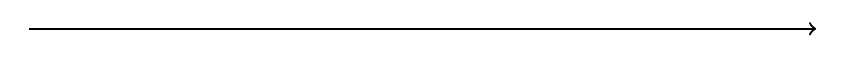
\begin{tikzpicture}[scale=1]
			\draw[->,thick](-4,0) --(6,0);
		\end{tikzpicture}\\
		%
		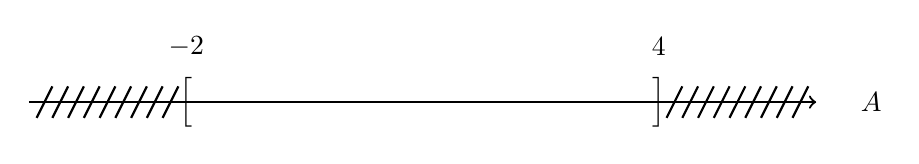
\begin{tikzpicture}[scale=1]
			\draw[->,thick](-4,0) --(6,0) node at (-2,0.7){$-2$} node at (4,0.7){$4$} node at (-2,0) {$\Big [$} node at (4,0) {$\Big ]$}node at (6.7,0){$A$};
			\foreach \b in {-3.8,-3.6,...,-2.2} {\draw[ thick](\b-0.1,-0.2)--(\b+0.1,0.2);}
			\foreach \b in {4.2,4.4,...,5.8} {\draw[ thick](\b-0.1,-0.2)--(\b+0.1,0.2);}
		\end{tikzpicture}\\
		%
		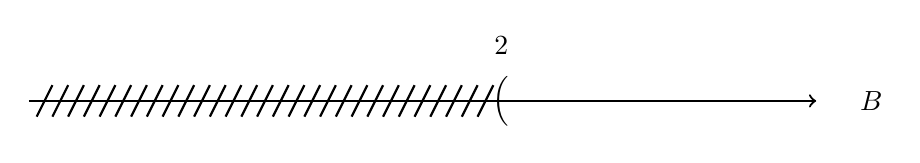
\begin{tikzpicture}[scale=1]
			\draw[->,thick](-4,0) --(6,0) node at (2,0.7){$2$} node at (2,0) {$\Big ($}node at (6.7,0){$B$};
			\foreach \b in {-3.8,-3.6,...,1.8} {\draw[ thick](\b-0.1,-0.2)--(\b+0.1,0.2);}
		\end{tikzpicture}\\
		%
		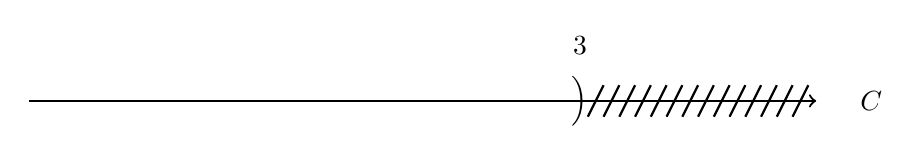
\begin{tikzpicture}[scale=1]
			\draw[->,thick](-4,0) --(6,0) node at (3,0.7){$3$} node at (3,0) {$\Big )$}node at (6.7,0){$C$};
			\foreach \b in {3.2,3.4,...,5.8} {\draw[ thick](\b-0.1,-0.2)--(\b+0.1,0.2);}
		\end{tikzpicture}\\
		%
		\begin{enumerate}
			\item $A\cap B=\left(2;4\right], B\cap C=\left(2;3\right)$.
			\item $\mathbb{R}\cap A=\left[-2;4 \right],\mathbb{R}\cap B=\left(2;+\infty \right)$.
		\end{enumerate}
	}
\end{bt}
\begin{bt}%[Huỳnh Quy]%[0D1B4-2]
	Cho hai tập hợp $A=\lbrace x\in \mathbb{R}\vert  x \leq 2 \rbrace$, $B=\lbrace x\in \mathbb{R}\vert -2< x \rbrace$. Tìm $A\setminus B, B\setminus A$.
	\loigiai{
		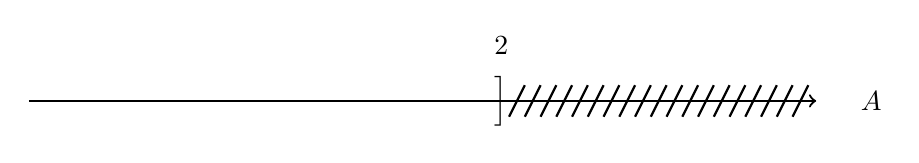
\begin{tikzpicture}[scale=1]
			\draw[->,thick](-4,0) --(6,0) node at (2,0.7){$2$} node at (2,0) {$\Big ]$}node at (6.7,0){$A$};
			\foreach \b in {2.2,2.4,...,5.8} {\draw[ thick](\b-0.1,-0.2)--(\b+0.1,0.2);}
		\end{tikzpicture}\\
		%
		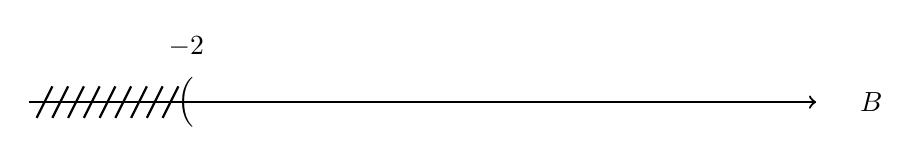
\begin{tikzpicture}[scale=1]
			\draw[->,thick](-4,0) --(6,0) node at (-2,0.7){$-2$} node at (-2,0) {$\Big ($} node at (6.7,0){$B$};
			\foreach \b in {-3.8,-3.6,...,-2.2} {\draw[ thick](\b-0.1,-0.2)--(\b+0.1,0.2);}
		\end{tikzpicture}\\
		$\Rightarrow A\setminus B=\left(-\infty;-2 \right], B\setminus A=\left(2;+\infty \right)$.}
\end{bt}
\begin{bt}%[Huỳnh Quy]%[0D1B4-2] 
	Cho $A=\left[-2;4\right],B=\left(2;+\infty\right),C=(-\infty;3)$. Xác định các tập hợp sau đây và biểu diễn chúng trên trục số.
	\begin{enumerate}
		\item $A\setminus B, B\setminus A$.
		\item $\mathbb{R}\setminus A,\mathbb{R}\setminus B, \mathbb{R}\setminus  C$.
	\end{enumerate}
	\loigiai{
		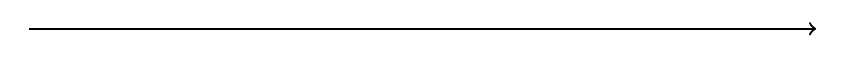
\begin{tikzpicture}[scale=1]
			\draw[->,thick](-4,0) --(6,0);
		\end{tikzpicture}\\
		%
		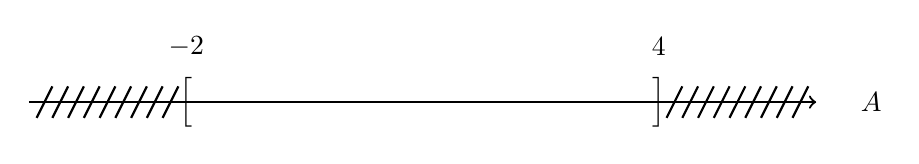
\begin{tikzpicture}[scale=1]
			\draw[->,thick](-4,0) --(6,0) node at (-2,0.7){$-2$} node at (4,0.7){$4$} node at (-2,0) {$\Big [$} node at (4,0) {$\Big ]$}node at (6.7,0){$A$};
			\foreach \b in {-3.8,-3.6,...,-2.2} {\draw[ thick](\b-0.1,-0.2)--(\b+0.1,0.2);}
			\foreach \b in {4.2,4.4,...,5.8} {\draw[ thick](\b-0.1,-0.2)--(\b+0.1,0.2);}
		\end{tikzpicture}\\
		%
		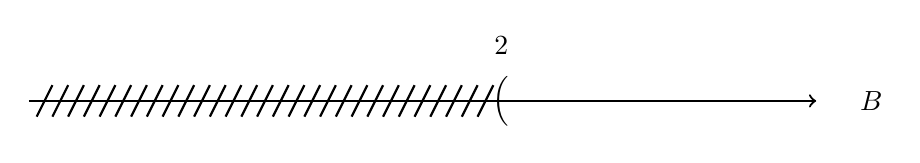
\begin{tikzpicture}[scale=1]
			\draw[->,thick](-4,0) --(6,0) node at (2,0.7){$2$} node at (2,0) {$\Big ($}node at (6.7,0){$B$};
			\foreach \b in {-3.8,-3.6,...,1.8} {\draw[ thick](\b-0.1,-0.2)--(\b+0.1,0.2);}
		\end{tikzpicture}\\
		%
		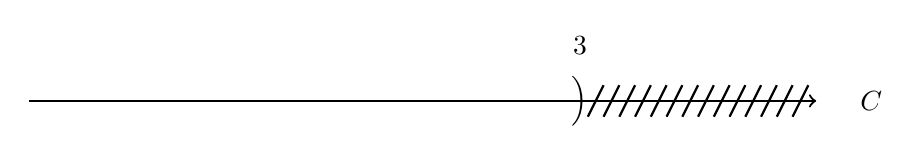
\begin{tikzpicture}[scale=1]
			\draw[->,thick](-4,0) --(6,0) node at (3,0.7){$3$} node at (3,0) {$\Big )$}node at (6.7,0){$C$};
			\foreach \b in {3.2,3.4,...,5.8} {\draw[ thick](\b-0.1,-0.2)--(\b+0.1,0.2);}
		\end{tikzpicture}
		%
		\begin{enumerate}
			\item $A\setminus B=\left[-2;2\right], B\setminus A=\left(4;+\infty\right)$.
			\item $\mathbb{R}\setminus A=\left(\infty;-2\right)\cup\left(4;+\infty \right),\mathbb{R}\setminus B=\left(-\infty;2\right], \mathbb{R}\setminus  C=\left[3;+\infty \right)$.
		\end{enumerate}
	}
\end{bt}
\begin{dang}{Ứng dụng thực tế các phép toán tập hợp}
\end{dang}
\subsubsection{Ví dụ minh hoạ}
\begin{vd}%[BG10-2022]%[Đỗ Văn Dự]%[0D1Y3-3]
	Cho $A$ là tập hợp các học sinh giỏi Toán của trường THPT X và $B$ là tập hợp học sinh giỏi Văn của trường này. Hãy mô tả các học sinh thuộc tập hợp sau\begin{enumEX}{3} 
			\item $A\cup B$.
			\item $A\cap B$.
			\item $A\setminus B$.
			\item $B\setminus A$.
			\item $\left(A\cup B\right)\setminus \left(A\cap B\right)$.
	\end{enumEX}
	\loigiai{
		\immini{
			\begin{enumerate}
				\item $A\cup B$ là tập hợp các học sinh giỏi Toán hoặc giỏi Văn của trường.
				\item $A\cap B$ là tập hợp các học sinh giỏi cả hai môn Toán và Văn của trường.
				\item $A\setminus B$ là tập hợp các học sinh chỉ giỏi Toán, không giỏi Văn.
				\item $B\setminus A$ là tập hợp các học sinh chỉ giỏi Văn, không giỏi Toán.		
				\item $\left(A\cup B\right)\setminus \left(A\cap B\right)$ là tập hợp các học sinh chỉ giỏi Toán hoặc giỏi Văn của trường.	
			\end{enumerate}
		}
		{\begin{tikzpicture}[scale=1, line join=round, line cap=round]	
				\coordinate (A) at (-1.2,0);
				\coordinate (B) at (0.8,0);
				\begin{scope}
					\clip[rotate=20] (A) ellipse (2cm and 1cm); %cat theo elip A
					\fill[rotate=30,pattern=north west lines] (B) ellipse (2cm and 1cm); %to elip B nhung bi cat mat theo phan giao voi elip A
				\end{scope}
				\draw[rotate=20] (A) ellipse (2cm and 1cm) node[fill=white,above]{$A\setminus B$}; %ve lai elip A
				\draw[rotate=30] (B) ellipse (2cm and 1cm) node[fill=white,above,right]{$B\setminus A$}; %ve lai elip B
				\path (-0.2,0.2) node[below]{$A\cap B$};
		\end{tikzpicture}}
	}
\end{vd}
\begin{vd}%[BG10-2022]%[Đỗ Văn Dự]%[0D1B3-3]
	Trong kì thi học sinh giỏi cấp trường, lớp 10C1 có $45$ học sinh trong đó có  $17$ bạn đạt học sinh giỏi Văn, $25$ bạn đạt học sinh giỏi Toán và $13$ bạn học sinh không đạt học sinh giỏi. Tìm số học sinh giỏi cả Văn và Toán của lớp 10C1.
	\loigiai{
		\immini{
			\begin{itemize}			
				\item Gọi $A$, $B$ theo thứ tự là tập hợp các học sinh giỏi Văn và giỏi Toán của lớp. 
				Theo đề ta có $n(A)=17$, $n(B)=25$, $n(A \cup B)= 45-13=32$.
				\item Số học sinh giỏi cả Văn và Toán là $$n(A \cap B )=n(A) + n(B) - n(A \cup B)=25+17-32=10.$$
			\end{itemize}
		}
		{	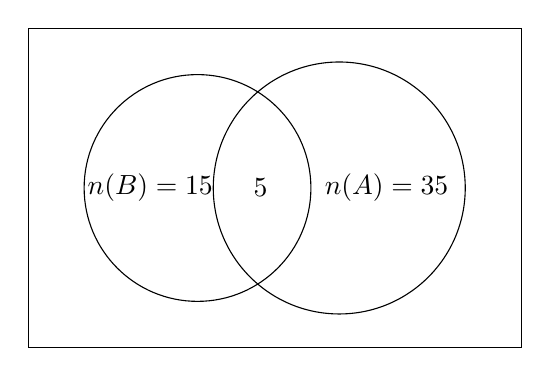
\begin{tikzpicture}[scale=.8]
				\def\radius{2cm}	
				\coordinate (ceni);
				\coordinate[xshift=.9*\radius] (cenii);
				
				\draw (ceni) circle (.9*\radius);
				\draw (cenii) circle (\radius);
				\draw  ([xshift=-25pt,yshift=15pt]current bounding box.north west) 
				rectangle ([xshift=25pt,yshift=-15]current bounding box.south east);
				
				\node[xshift=-.3*\radius] at (ceni) {$n(B)=15$};
				\node[xshift=.3*\radius] at (cenii) {$n(A)=35$};
				\node[xshift=.4*\radius] at (ceni) {$5$};
	\end{tikzpicture}}}
\end{vd}
\begin{vd}%[BG10-2022]%[Đỗ Văn Dự]%[0D1B3-3]
	Một lớp học có $ 50 $ học sinh trong đó có $ 30 $ em biết chơi bóng chuyền, $25$ em biết chơi bóng đá, $ 10 $ em biết chơi cả bóng đá và bóng chuyền. Hỏi có bao nhiêu em không biết chơi môn nào trong hai môn ở trên?
	\loigiai{
		Gọi tập $A$ là tập hợp các học sinh biết chơi bóng chuyền.
		\\Tập $B$ là tập hợp các học sinh biết chơi bóng đá.
		\\Khi đó số học sinh biết chơi ít nhất một trong hai môn bóng chuyền hoặc bóng đá là 
		$$n(A \cup B)=n(A)+n(B)-n(A \cap B)=30+25-10=45.$$
		Vậy số học sinh không biết chơi môn nào là $50-45=5$. 		
	}	
\end{vd}
\begin{vd}%[BG10-2022]%[Đỗ Văn Dự]%[0D1B3-3]
	Trong số $45$ cán bộ được triệu tập để chuẩn bị công tác cho một cuộc hội nghị quốc tế có $25$ cán bộ phiên dịch tiếng Anh, $15$ cán bộ phiên dịch tiếng Pháp, trong đó có $10$ cán bộ vừa phiên dịch được tiếng Anh, vừa phiên dịch được tiếng Pháp. Hỏi
	\begin{enumerate}
		\item Nhóm có bao nhiêu cán bộ được cấp thẻ đỏ, biết rằng muốn được cấp thẻ đỏ cán bộ đó phải phiên dịch được tiếng Anh hoặc phiên dịch được tiếng Pháp.
		\item Nhóm có bao nhiêu cán bộ không phiên dịch được tiếng Anh và không phiên dịch được tiếng Pháp.
	\end{enumerate}
	\loigiai{
		Gọi $A$, $B$ theo thứ tự là tập hợp các cán bộ phiên dịch tiếng Anh và tập hợp các các bộ phiên dịch tiếng Pháp. 
		Theo đề ta có $n(A)=25$, $n(B)=15$, $n(A \cap B)= 10$.
		\begin{enumerate}				
			\item Tập hợp các cán bộ được cấp thẻ đỏ là $A\cup B$.\\
			Vậy số cán bộ được cấp thẻ đỏ là $n(A \cup B)=n(A)+n(B)-n(A \cap B)=25+15-10=30$.
			\item Tập hợp các cán bộ của nhóm không phiên dịch được tiếng Anh và tiếng Pháp chính là số cán bộ không được cấp thẻ đỏ.\\
			Vậy số cán bộ đó là $45-30=15$.
	\end{enumerate}}
\end{vd}
\begin{vd}%[BG10-2022]%[Đỗ Văn Dự]%[0D1B3-3]
	Lớp $10A$ có $15$ bạn thích môn Văn, $20$ bạn thích môn Toán. Trong số các bạn thích văn hoặc toán có $8$ bạn thích cả $2$ môn. Trong lớp vẫn còn $10$ bạn không thích môn nào trong $2$ môn Văn và Toán. Hỏi lớp $10A$ có bao nhiêu học sinh?
	\loigiai{Ta sử dụng sơ đồ Ven.		
		\begin{center}
			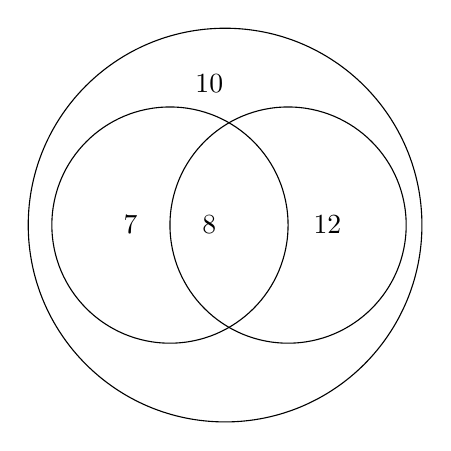
\begin{tikzpicture}
				\draw[] (0.7,0) circle ( 2.5cm);
				\draw[] (0,0) circle ( 1.5cm);
				\draw (1.5,0) circle ( 1.5 cm);
				\draw (-0.5,0) node {$7$};
				\draw (2,0) node {$12$};
				\draw (0.5,0) node {$8$};
				\draw (0.5,1.8) node {$10$};
			\end{tikzpicture}
		\end{center}
		\begin{itemize}
			\item Hình tròn lớn ngoài cùng thể hiện số học sinh cả lớp.\\
			Như vậy, ta có:\\
			\item	Số bạn chỉ thích Văn là $ 15-8=7$(bạn).\\
			\item	Số bạn chỉ thích Toán là $20-8=12$(bạn).\\
			\item	Số học sinh cả lớp là tổng các phần không giao nhau: $7+8+12+10=37$.
		\end{itemize}
	}
\end{vd}

\begin{vd}%[BG10-2022]%[Đỗ Văn Dự]%[0D1B3-3]
	Một lớp có $40$ học sinh, mỗi học sinh đều đăng ký chơi ít nhất $1$ trong $2$ môn thể thao là bóng đá hoặc cầu lông. Có $30$ học sinh có đăng ký môn bóng đá, $25$ học sinh có đăng ký môn cầu lông. Hỏi có bao nhiêu em đăng ký cả $2$ môn.
	\loigiai{
		Gọi $A$ là tập hợp các học sinh đăng kí chơi bóng đá, $B$ là tập học sinh đăng kí chơi cầu lông thì $A\cap B$ là tập hợp các học sinh đăng kí chơi cả hai môn.\\	
		Vậy số học sinh đăng kí chơi cả hai môn là 
		$n(A \cap B)=n(A)+n(B)-n(A \cup B)=30+25-40=15$. }
\end{vd}

\begin{vd}%[BG10-2022]%[Đỗ Văn Dự]%[0D1B3-3]
	Ở xứ sở của thần Thoại ngoài các vị thần thì còn có các sinh vật gồm $27$ con người, $311$ con yêu quái một mắt, $205$ con yêu quái tóc rắn và yêu quái vừa một mắt vừa tóc rắn. Tìm số yêu quái vừa một mắt vừa tóc rắn biết có tổng số sinh vật là 500 con.
	\loigiai{
		\begin{itemize}
			\item Số sinh vật không phải con người là $500-27=473$ (con).
			\item Gọi $A$, $B$ lần lượt là tập hợp yêu quái một mắt và yêu quái tóc rắn. Khi đó $n(A)=311$,  $n(B)=205$, $n(A \cup B)=473$.
			\item Vậy số yêu quái vừa một mắt vừa tóc rắn là $|A \cap B| =311+205-473=43$.
		\end{itemize}
	}
\end{vd}

\begin{vd}%[BG10-2022]%[Đỗ Văn Dự]%[0D1B3-3]
	Mỗi học sinh của lớp $10A$ đều chơi bóng đá hoặc bóng chuyền. Biết rằng có $25$ bạn chơi bóng đá, $20$ bạn chơi bóng chuyền và $10$ bạn chơi cả $2$ môn thể thao. Hỏi lớp $10A$ có bao nhiêu học sinh.
	\loigiai{
		Gọi $A$ là tập hợp các học sinh chơi bóng đá, $B$ là tập các học sinh chơi bóng chuyền. Do đó $A\cap B$ là tập các học sinh chơi cả hai môn.\\
		Theo đề $n(A)=25$, $n(B)=20$, $|A \cap B| =10$.\\
		Vậy số học sinh cả lớp là $|A \cup B| =n(A)+n(B)-n(A \cap B)=25+20-10=35$.}
\end{vd}

\begin{vd}%[BG10-2022]%[Đỗ Văn Dự]%[0D1B3-3]
	Lớp 10A có $45$ học sinh, có $15$ học sinh giỏi và $20$ học sinh xếp hạnh kiểm tốt, trong đó có $10$ bạn vừa học giỏi vừa xếp hạnh kiểm tốt. Các học sinh được học sinh giỏi hoặc hạnh kiểm tốt đều được khen thưởng. Số học sinh được khen thưởng của lớp 10A là là bao nhiêu?
	\loigiai{
		Gọi $A$ là tập hợp các học sinh giỏi, 
		$B$ là tập hợp các học sinh xếp hạnh kiểm tốt.\\
		Khi đó số học sinh được khen thưởng là $n(A \cup B)$.\\
		Vậy số học sinh được khen thưởng là 
		$n(A \cup B)=n(A)+n(B)-n(A \cap B)=15+20-10=25.$		
	}
\end{vd}

\begin{vd}%BT6%[Nguyễn Thành Tuấn]%[0D1K3-3]
	Kết quả thi học kì một của một trường THPT có $48$ thí sinh giỏi môn Toán, $37$ thí sinh giỏi môn Vật Lí,$42$ thí sinh giỏi môn Văn. Biết rằng có $75$ thí sinh giỏi môn Toán hoặc môn Vật lí, $76$ thí sinh giỏi  môn Toán hoặc môn Văn, $66$ thí sinh giỏi môn Vật lí hoặc môn Văn và có $4$ thí sinh giỏi cả ba môn. Hỏi 
	\begin{enumerate}
		\item có bao nhiêu học sinh chỉ giỏi 1 môn.
		\item có bao nhiêu học sinh chỉ giỏi 2 môn.
		\item có bao nhiêu học sinh giỏi ít nhất 1 môn.
	\end{enumerate}
	\loigiai{		
		Gọi $A$, $B$, $C$ theo thứ tự là tập hợp các học sinh giỏi Toán, giỏi Lí và giỏi Văn. Theo đề ta có
		\begin{itemize}
			\item Số học sinh giỏi Toán và Lí là $$n(A \cap B)=n(A)+n(B)-n(A \cup B)=48+37-75=10.$$	
			\item Số học sinh giỏi Toán và Văn là $$n(A \cap C)=n(A)+n(C)-n(A\cup C)=48+42 - 76 = 14 .$$	
			\item Số học sinh giỏi Lí và Văn là $$n(B \cap C)=n(B)+n(C)-n(B\cup C)= 42+37-66=13 .$$	
			\item Số học sinh chỉ giỏi môn Toán $48-10-14+4=28 $.	
			\item Số học sinh chỉ giỏi môn Lí $37-10-13+4=18 $.	
			\item Số học sinh chỉ giỏi môn Văn $42-13-14+4=19 $.
		\end{itemize}
		\begin{center}
			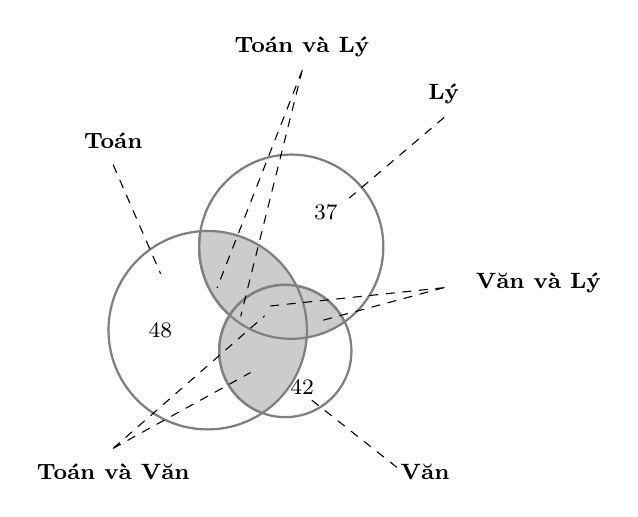
\begin{tikzpicture}[scale=0.6,>=stealth, font=\footnotesize, line join=round, line cap=round]	
				\def\firstcircle{(0,0) circle (2.1cm)}
				\def\secondcircle{(45:2.5cm) circle (1.95cm)}
				\def\thirdcircle{(-15:1.7cm) circle (1.4cm)}
				\colorlet{circle edge}{black!50}
				\colorlet{circle area}{black!20}
				\tikzset{filled/.style={fill=circle area, draw=circle edge, thick},
					outline/.style={draw=circle edge, thick}}
				\draw \firstcircle;
				\draw \secondcircle;
				\draw \thirdcircle;
				\begin{scope}
					\clip \firstcircle;
					\fill[filled] \secondcircle;
				\end{scope}
				\begin{scope}
					\clip \firstcircle;
					\fill[filled] \thirdcircle;
				\end{scope}
				\begin{scope}
					\clip \secondcircle;
					\fill[filled] \thirdcircle;
				\end{scope}  
				\node at (-1,0){48};  
				%\node at (0.5,1){3}; 
				%	\node at (1.2,0.3){1};  
				%	\node at (2.3,0.3){1};      
				%	\node at (1,-0.5){2};   
				\node at (2,-1.2){42};     
				\node at (2.5,2.5){37}; 
				\draw[outline] \firstcircle
				\secondcircle  \thirdcircle;    
				\node at (-2,4) {\textbf{Toán}};
				\node at (2,6) {\textbf{Toán và Lý}};
				\node at (5,5) {\textbf{Lý}};
				\node at (7,1) {\textbf{Văn và Lý}};   
				\node at (4.6,-3) {\textbf{Văn}};
				\node at (-2,-3) {\textbf{Toán và Văn}};
				\draw[dashed] (-2,3.5) -- (-1,1.2) 
				(2,5.5) -- (0.7,0.3) 
				(2,5.5) -- (0.2,0.9)
				(5,4.5) -- (3,2.8)
				(5,0.9) -- (1.2,0.5)
				(5,0.9) -- (2.4,0.2)
				(4,-2.9) -- (2.1,-1.4)
				(-2,-2.5) -- (1.2,0.3)
				(-2,-2.5) -- (0.9,-0.9)	;
		\end{tikzpicture}	
		\end{center}
		
		\begin{enumerate}	
			\item Số học sinh chỉ giỏi đúng 1 môn là $28+18+19=65$. 
			\item Số học sinh chỉ giỏi đúng 2 môn là $10+14+13-4\cdot2=25 $. 
			\item Số học sinh giỏi ít nhất một môn là $65+25+4=94$.
		\end{enumerate}
	}
\end{vd}
\begin{vd}%[BG10-2022]%[Đỗ Văn Dự]%[0D1K3-3]
	Một nhóm học sinh giỏi các bộ môn: Anh, Toán, Văn. Có $18$ em giỏi Văn, $10$ em giỏi Anh, $12$ em giỏi Toán, $3$ em giỏi Văn và Toán, $4$ em giỏi Toán và Anh, $5$ em giỏi Văn và Anh, $2$ em giỏi cả ba môn. Hỏi nhóm đó có bao nhiêu em?
	\loigiai{
		Gọi $A$ là tập hợp những học sinh giỏi Anh,
		$T$ là tập hợp những học sinh giỏi toán,
		$V$ là tập hợp những học sinh giỏi Văn.
		Ta có\\
		$\bullet$ $n\left( V \right)=18,\; n\left( A \right)=10$,\; $n\left( T \right)=12$,\; 
		$n(V\cap T)=3,\;n(T\cap A)=4,\;n(V\cap A)=5$,\; $n(A\cap B\cap C)=2$.\\
		$\bullet$  $\begin{aligned}[t] n(V\cup A\cup T)&=n\left( V \right)+n\left( A \right)+n\left( T \right)-\left[ n(V\cap A)+n(A\cap T)+n(T\cap V) \right]+n\left( V\cap A\cap T \right)\\ &=
		18+10+12-\left[ 3+4+5 \right]+2=30 \end{aligned}$.\\
		Vậy nhóm đó có 30 em.}
\end{vd}

\begin{vd}%[BG10-2022]%[Đỗ Văn Dự]%[0D1K3-3]
	Trong số $42$ học sinh của lớp 10A có $13$ bạn được xếp loại học lực giỏi, $22$ bạn được xếp loại hạnh kiểm tốt, trong đó $7$ bạn vừa học lực giỏi, vừa có hạnh kiểm tốt. Hỏi lớp 10A có bao nhiêu bạn được khen thưởng? Biết rằng muốn được khen thưởng thì bạn đó phải có học lực giỏi hoặc có hạnh kiểm tốt.
	\loigiai{
		Gọi tập hợp các học sinh học lực giỏi là $G$, tập hợp các bạn học sinh hạnh kiểm tốt là $T$. Khi đó tập hợp các bạn học sinh vừa có học lực giỏi là, vừa có hạnh kiểm tốt là $G\cap T$, tập hợp các bạn học sinh đạt học lực giỏi hoặc hạnh kiểm tốt là $G\cup T$. Ta có \\
		$n(G)=13$, $n(T)=22$, $n(G\cap T)=7$.\\
		$n(G\cup T)=n(G)+n(T)-n(G\cap T)=13+22-7=28.$}
\end{vd}

\begin{vd}%[BG10-2022]%[Đỗ Văn Dự]%[0D1K3-3]
	Một nhóm học sinh giỏi các bộ môn: Anh, Toán, Văn. Có $ 18 $ em giỏi Văn, $ 10 $ em giỏi Anh, $ 12 $ em giỏi Toán, $ 3 $ em giỏi Văn và Toán, $ 4 $ em giỏi Toán và Anh, $ 5 $ em giỏi Văn và Anh, $ 2 $ em giỏi cả ba môn. Hỏi nhóm đó có bao nhiêu em?
	\loigiai{
		\begin{center}
			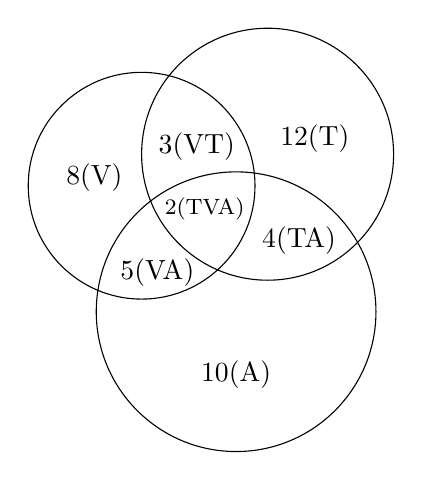
\begin{tikzpicture}[scale=.8]
				\def\radius{2cm}	
				\coordinate (ceni);
				\coordinate[xshift=.8*\radius, yshift=.2*\radius] (cenii);
				\coordinate[xshift=.6*\radius,yshift=-.8*\radius] (ceniii);
				\draw (ceni) circle (.9*\radius);
				\draw (cenii) circle (\radius);
				\draw (ceniii) circle (1.11*\radius);
				
				\node[xshift=-.3*\radius, yshift=.05*\radius] at (ceni) {$8$(V)};
				\node[xshift=.35*\radius, yshift=.25*\radius] at (ceni) {$3$(VT)};
				\node[xshift=.1*\radius, yshift=-.55*\radius] at (ceni) {$5$(VA)};
				\node[xshift=.4*\radius, yshift=-.15*\radius] at (ceni) {{\footnotesize $2$(TVA)}};
				\node[xshift=.2*\radius, yshift=-.55*\radius] at (cenii) {$4$(TA)};
				\node[xshift=1.1*\radius,yshift=.3*\radius] at (ceni) {$12$(T)};
				\node[yshift=-.4*\radius] at (ceniii) {$10$(A)};
			\end{tikzpicture}
		\end{center}
		Ký hiệu $ A $ là tập hợp những học sinh giỏi Anh,\\
		$ T $ là tập hợp những học sinh giỏi Toán,\\
		$ V $ là tập hợp những học sinh giỏi Văn.\\
		$\bullet$ $n(V)=18,\; n(A)=10,\; n(T)=12$,\\
		$\bullet$ $n(T \cap V)=3,\; n(T \cap A)=4,\; n(V \cap A)=5, n(A \cap B \cap C)=2$.\\
		Số học sinh của nhóm là
		\begin{eqnarray*}
			n(V \cup A \cup T)&=&n(V)+n(A)+n(T)-n(V \cap A)-n(T \cap A)-n(T \cap V)+n(A \cap B \cap C)\\
			&=&18+10+12-(3+4+5)+2=30.
		\end{eqnarray*}
		Vậy nhóm đó có $ 30 $ em.
	}
\end{vd}

\begin{vd}%[BG10-2022]%[Đỗ Văn Dự]%[0D1K3-3]
	Có $44$ học sinh giỏi, mỗi em giỏi ít nhất một môn. Có $22$ em giỏi Văn, $25$ em giỏi Toán, $20$ em giỏi Anh. Có $8$ em giỏi đúng hai môn Văn, Toán; Có $7$ em giỏi đúng hai môn Toán, Anh; Có $6$ em giỏi đúng hai môn Anh, Văn. Hỏi có bao nhiêu em giỏi cả ba môn Văn, Toán, Anh?
	\loigiai{
		Ta có \\
		$n\left( V \right)=22,\;n\left( T \right)=25$,\; $n\left( A \right)=20$\\
		$n((V\cap T)\setminus A)=8,\;n((T\cap A)\setminus V)=7,\;n((V\cap A)\setminus T)=6,\; n(V\cup T\cup A)=44$.\\
		$n(V\cup A\cup T)=n\left( V \right)+n\left( A \right)+n\left( T \right)-n(V\cap A)-n(A\cap T)-n(T\cap V)+n\left( V\cap A\cap T \right)$\\
		$  \Leftrightarrow  44=22+20+25-6-7-8+4n\left( V\cap A\cap T \right)$.\\
		$\Rightarrow n\left( V\cap A\cap T \right)=1$.
	}
\end{vd}
\begin{vd}%[BG10-2022]%[Đỗ Văn Dự]%[0D1B3-3]
	Để thành lập đội tuyển học sinh giỏi khối $ 10 $, nhà trường tổ chức thi chọn các môn Toán, Văn, Anh trên tổng số $ 111 $ học sinh. Kết quả có: $ 70 $ học sinh giỏi Toán, $ 65 $ học sinh giỏi Văn, $ 62 $ học sinh giỏi Anh. Trong đó có $ 49 $ học sinh giỏi cả hai môn Văn và Toán, $ 32 $ học sinh giỏi cả hai môn Toán và Anh, $ 34 $ học sinh giỏi cả hai môn Văn và Anh. Xác định số học sinh giỏi cả ba môn Văn, Toán, Anh. Biết rằng có $ 6 $ học sinh không đạt yêu cầu cả ba môn.
	\loigiai{
		\immini
		{Có $ 111-6=105 $ học sinh thi đạt ít nhất $ 1 $ môn.\\
			Gọi $ A $ là số học sinh giỏi môn Toán và Tiếng Anh nhưng không giỏi Văn.\\
			Gọi $ B $ là số học sinh giỏi môn Toán và Văn nhưng không giỏi Tiếng Anh.\\
			Gọi $ C $ là số học sinh giỏi môn Văn và Tiếng Anh nhưng không giỏi Toán.\\
			Gọi $ D $ là số học sinh giỏi cả ba môn. Ta có hệ:\\
			$\begin{cases}
				B+D=49\\
				A+D=32\\
				C+D=34\\
				70+65+62-(A+B+C+2D)=105
			\end{cases}\\
			\Rightarrow 92=32-D+49-D+34-D+2D\\
			\Rightarrow D=23$.\\
			Vậy có $ 23 $ học sinh giỏi cả ba môn.
		}
		{
			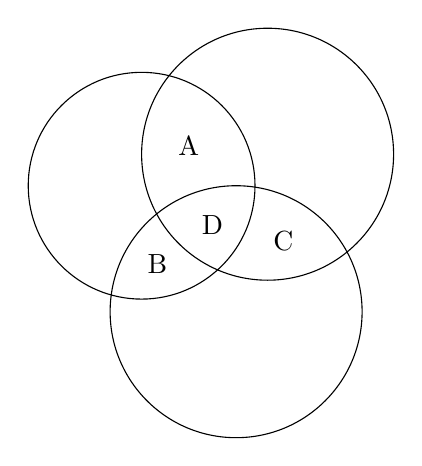
\begin{tikzpicture}[scale=.8]
				\def\radius{2cm}	
				\coordinate (ceni);
				\coordinate[xshift=.8*\radius, yshift=.2*\radius] (cenii);
				\coordinate[xshift=.6*\radius,yshift=-.8*\radius] (ceniii);
				\draw (ceni) circle (.9*\radius);
				\draw (cenii) circle (\radius);
				\draw (ceniii) circle (\radius);
				
				\node[xshift=.3*\radius, yshift=.25*\radius] at (ceni) {A};
				\node[xshift=.1*\radius, yshift=-.5*\radius] at (ceni) {B};
				\node[xshift=.45*\radius, yshift=-.25*\radius] at (ceni) {D};
				\node[xshift=.1*\radius, yshift=-.55*\radius] at (cenii) {C};
		\end{tikzpicture}}
	}
\end{vd}
\subsubsection{Bài tập tự luận}
\begin{bt}%[Huỳnh Quy]%[0D1B3-3]
	Mỗi học sinh của lớp $10A$ đều chơi bóng đá hoặc bóng chuyền. Biết rằng có $25$ bạn chơi bóng đá, $20$ bạn chơi bóng chuyền và $10$ bạn chơi cả $2$ môn thể thao. Hỏi lớp $10A$ có bao nhiêu học sinh.
	\loigiai{
		Ngoài sơ đồ Ven ta có thể dùng công thức số phần tử. Gọi $A$ là tập hợp các học sinh chơi bóng đá, $B$ là tập các học sinh chơi bóng chuyền. Do đó $A\cap B$ là tập các học sinh chơi cả hai môn. Ta có
		$$n(A)=25, n(B)=20, n(A \cap B) =10.$$
		Số học sinh cả lớp là số phần tử của tập $A \cup B$ nên $n(A \cup B) = 25+20-10=35$ (học sinh).
	}
\end{bt}
\begin{bt}%[Huỳnh Quy]%[0D1B3-3]
	Lớp $10{{B}_{1}}$ có $7$ học sinh giỏi Toán, $5$ học sinh giỏi Lý, $6$ học sinh giỏi Hóa, $3$ học sinh giỏi cả Toán và Lý, $4$ học sinh giỏi cả Toán và Hóa, $2$ học sinh giỏi cả Lý và Hóa, $1$ học sinh giỏi cả $3$ môn Toán, Lý, Hóa. Tính số học sinh giỏi ít nhất một môn (Toán, Lý, Hóa) của lớp $10{{B}_{1}}$.
	\loigiai{
		Ta dùng biểu đồ Ven để giải:
		\begin{center}
			\begin{tikzpicture}
				\def\firstcircle{(0,0) circle (1.5cm)}
				\def\secondcircle{(45:2.5cm) circle (2cm)}
				\def\thirdcircle{(-15:1.7cm) circle (1.4cm)}
				\colorlet{circle edge}{black!50}
				\colorlet{circle area}{black!20}
				\tikzset{filled/.style={fill=circle area, draw=circle edge, thick},
					outline/.style={draw=circle edge, thick}}
				\draw \firstcircle;
				\draw \secondcircle;
				\draw \thirdcircle;
				\begin{scope}
					\clip \firstcircle;
					\fill[filled] \secondcircle;
				\end{scope}
				\begin{scope}
					\clip \firstcircle;
					\fill[filled] \thirdcircle;
				\end{scope}
				\begin{scope}
					\clip \secondcircle;
					\fill[filled] \thirdcircle;
				\end{scope}  
				\node at (-1,0){1};  
				\node at (0.5,1){2}; 
				\node at (1,0.3){1};  
				\node at (2,0.3){1};      
				\node at (1,-0.5){3};   
				\node at (2,-1){1};     
				\node at (3,2.5){1}; 
				\draw[outline] \firstcircle
				\secondcircle  \thirdcircle;    
				\node at (-2,4) {\textbf{Toán}};
				\node at (2,6) {\textbf{Giỏi Toán + Lý}};
				\node at (5,5) {\textbf{Lý}};
				\node at (7,1) {\textbf{Giỏi Hóa + Lý}};   
				\node at (5,-3) {\textbf{Hóa}};
				\node at (-2,-3) {\textbf{Giỏi Toán + Hóa}};
				\draw[->] (-2,3.5) -- (-1,1.2) 
				(2,5.5) -- (0.7,0.3) 
				(2,5.5) -- (0.2,0.9)
				(5,4.5) -- (3.6,2.5)
				(5,0.9) -- (1.2,0.5)
				(5,0.9) -- (2.4,0.2)
				(4,-2.9) -- (2,-1.8)
				(-2,-2.5) -- (1.2,0)
				(-2,-2.5) -- (0.9,-0.9)
				;
			\end{tikzpicture}
		\end{center}
		Nhìn vào biểu đồ, số học sinh giỏi ít nhất $1$ trong $3$ môn là: $1+2+1+3+1+1+1=10$}
\end{bt}
\begin{bt}%[Huỳnh Quy]%[0D1B3-3]
	Lớp $10{{\text{A}}_{1}}$ có $7$ học sinh giỏi Toán, $5$ học sinh giỏi Lý, $6$ học sinh giỏi Hóa, $3$ học sinh giỏi cả Toán và Lý, $4$ học sinh giỏi cả Toán và Hóa, $2$ học sinh giỏi cả Lý và Hóa, $1$ học sinh giỏi cả $3$ môn Toán, Lý, Hóa. Tính số học sinh giỏi đúng hai môn học của lớp $10{{\text{A}}_{1}}$.
	\loigiai{
		\begin{center}
			\begin{tikzpicture}
				\def\firstcircle{(0,0) circle (1.5cm)}
				\def\secondcircle{(45:2.5cm) circle (2cm)}
				\def\thirdcircle{(-15:1.7cm) circle (1.4cm)}
				\colorlet{circle edge}{black!50}
				\colorlet{circle area}{black!20}
				\tikzset{filled/.style={fill=circle area, draw=circle edge, thick},
					outline/.style={draw=circle edge, thick}}
				\draw \firstcircle;
				\draw \secondcircle;
				\draw \thirdcircle;
				\begin{scope}
					\clip \firstcircle;
					\fill[filled] \secondcircle;
				\end{scope}
				\begin{scope}
					\clip \firstcircle;
					\fill[filled] \thirdcircle;
				\end{scope}
				\begin{scope}
					\clip \secondcircle;
					\fill[filled] \thirdcircle;
				\end{scope}  
				\node at (-1,0){1};  
				\node at (0.5,1){2}; 
				\node at (1,0.3){1};  
				\node at (2,0.3){1};      
				\node at (1,-0.5){3};   
				\node at (2,-1){1};     
				\node at (3,2.5){1}; 
				\draw[outline] \firstcircle
				\secondcircle  \thirdcircle;    
				\node at (-2,4) {\textbf{Toán}};
				\node at (2,6) {\textbf{Giỏi Toán + Lý}};
				\node at (5,5) {\textbf{Lý}};
				\node at (7,1) {\textbf{Giỏi Hóa + Lý}};   
				\node at (5,-3) {\textbf{Hóa}};
				\node at (-2,-3) {\textbf{Giỏi Toán + Hóa}};
				\draw[->] (-2,3.5) -- (-1,1.2) 
				(2,5.5) -- (0.7,0.3) 
				(2,5.5) -- (0.2,0.9)
				(5,4.5) -- (3.6,2.5)
				(5,0.9) -- (1.2,0.5)
				(5,0.9) -- (2.4,0.2)
				(4,-2.9) -- (2,-1.8)
				(-2,-2.5) -- (1.2,0)
				(-2,-2.5) -- (0.9,-0.9)
				;
			\end{tikzpicture}
		\end{center}
		Dựa vào biểu đồ ven trên, ta có số học sinh giỏi đúng hai môn học là $2+1+3=6$}
\end{bt}

\subsection{Bài tập trắc nghiệm}
\Opensolutionfile{ans}[ans/ans-0D1-2-TN]
\begin{ex}%[Bài giảng Toán 10 - 2022]%[Nhật Thiện]%[0D1Y3-1]
	Cho hai tập hợp $X=\{1;3;5;8\}$, $Y=\{3;5;7;9\}$. Tập hợp $X\cup Y$ bằng tập hợp nào sau đây?
	\choice
	{$\{1;3;5\}$}
	{$\{3;5\}$}
	{$\{1;7;9\}$}
	{\True $\{1;3;5;7;8;9\}$}
	\loigiai{
		Ta có $X\cup Y=\{1;3;5;7;8;9\}$.
	}
\end{ex}
\begin{ex}%[Bài giảng Toán 10 - 2022]%[Nhật Thiện]%[0D1Y3-2]
	Cho hai tập hợp $A=\{1;2;3;4;5\}$ và $B=\{0;2;4;6;8\}$. Tìm $A\setminus B$.
	\choice
	{$A\setminus B=\{2;4\}$}
	{\True $A\setminus B=\{1;3;5\}$}
	{$A\setminus B=\{0;1;3;5\}$}
	{$A\setminus B=\{0;6;8\}$}
	\loigiai{
		Ta có $A\setminus B=\{1;3;5\}$.
	}
\end{ex}
\begin{ex}%[Bài giảng Toán 10 - 2022]%[Nhật Thiện]%[0D1B3-1]
	Cho hai tập hợp $ A=\left\lbrace x\in \mathbb{R}\,\mid\,(2x-x^2)(x-1)=0 \right\rbrace$, $ B=\left\lbrace n \in \mathbb{N}\,\mid\,0<n^2<10 \right\rbrace$. Chọn mệnh đề đúng?
	\choice
	{\True $A \cap B =\left\lbrace 1;2 \right\rbrace $}
	{$A \cap B =\left\lbrace 2 \right\rbrace $}
	{ $A \cap B =\left\lbrace 0;1;2;3 \right\rbrace $}
	{$A \cap B =\left\lbrace 0;3 \right\rbrace $}
	\loigiai{
		Ta có
		\begin{itemize}
			\item $ (2x-x^2)(x-1)=0\Leftrightarrow \hoac{& x=0 \\ &x=1\\&x=2 }\Rightarrow A=\left\lbrace 0;1;2 \right\rbrace  $.
			\item  $ B= \left\lbrace 1;2;3 \right\rbrace$.
		\end{itemize}
		Suy ra $ A\cap B= \left\lbrace 1;2 \right\rbrace$.}
\end{ex}
\begin{ex}%[Bài giảng Toán 10 - 2022]%[Nhật Thiện]%[0D1B3-1]
	Cho các tập hợp $A=\left\{ x\in \mathbb{N} \ | \ (4-x^2)(x^2-5x+4)=0 \right\}; B = \left\{ x\in \mathbb{Z} \ | \ x \text{ là ước của } 4 \right\}$. Tập hợp $A \cap B$ là
	\choice
	{$\{-2,1,2,4\}$}
	{\True $\{1,2,4\}$}
	{$\{2,4\}$}
	{$\{-4,-2,-1,1,2,4\}$}
	\loigiai{
		Ta có $(4-x^2)(x^2-5x+4)=0 \Leftrightarrow \hoac{&4-x^2=0\\&x^2-5x+4=0} \Leftrightarrow \hoac{&x=2\\&x=-2\\&x=1\\&x=4.}$\\
		Vì $x\in \mathbb{N}$ nên $x \in \{1,2,4\}$.\\
		Do đó $A=\{1,2,4\} \quad (1)$.\\
		Ta có các ước của $4$ là $\pm 1, \pm 2, \pm 4$.\\
		Do đó $B=\{-4,-2,-1,1,2,4\} \quad (2)$.\\
		Từ $(1), (2)$ ta có $A \cap B = \{1,2,4\}$.
	}
\end{ex}
\begin{ex}%[Bài giảng Toán 10 - 2022]%[Nhật Thiện]%[0D1Y4-2]
	Cho hai tập hợp $A = \left(-5;7\right)$ và $B = \left(1;+\infty\right)$. Tìm $A\setminus B$.
	\choice
	{\True $A\setminus B = \left(-5;1\right]$}
	{$A\setminus B = \left(-5;1\right)$}
	{$A\setminus B = \left[7;+\infty\right)$}
	{$A\setminus B = \left(7;+\infty\right)$}
	\loigiai{
		Ta có $A\setminus B = \left(-5;1\right]$.
	}
\end{ex}
\begin{ex}%[Bài giảng Toán 10 - 2022]%[Nhật Thiện]%[0D1Y4-2]
	Cho hai tập hợp $A=\left[ -2;4\right)$ và $B=\left(0;+\infty\right)$. Tìm khẳng định đúng.
	\choice
	{$A\cup B=\left(4;+\infty\right)$}
	{\True $A\cap B=\left(0;4\right)$}
	{$B\setminus A=\left[ -2;+\infty\right)$}
	{$A\setminus B=\left[ -2;0\right)$}
	\loigiai{
		$A\cup B=[-2;+\infty) \rightarrow $ loại.\\
		$A\cap B = (0;4) \rightarrow$ chọn.\\
		$B\setminus A = [4;+\infty) \rightarrow$ loại.\\
		$A\setminus B = [-2;0] \rightarrow$ loại.
	}
\end{ex}
\begin{ex}%[Bài giảng Toán 10 - 2022]%[Nhật Thiện]%[0D1B3-2]
	Cho $A$ là tập hợp các hình thoi, $B$ là tập hợp các hình chữ nhật và $C$ là tập hợp các hình vuông. Khi đó
	\choice
	{\True $A\cap B=C $}
	{$A\setminus B=C$}
	{$B\setminus A=C$}
	{$A\cup B=C$}
	\loigiai{
		Ta có hình thoi có hai cạnh kề vuông góc khi và chỉ khi nó là hình vuông.\\
		Hình chữ nhật có hai cạnh kề bằng nhau khi và chỉ khi nó là hình vuông.
	}
\end{ex}
\begin{ex}%[Bài giảng Toán 10 - 2022]%[Nhật Thiện]%[0D1B3-2]
	Cho hai tập hợp $M=\{1;2;3;5\}$ và $N=\{2;6;-1\}$. Xét các khẳng định
	\begin{enumEX}[(I)]{3}
		\item $M\cap N=\{2\}$
		\item $N\setminus M=\{1;3;5\}$
		\item $M\cup N=\{1;2;3;5;6;-1\}.$
	\end{enumEX}
	Có bao nhiêu khẳng định đúng trong ba khẳng định nêu trên?
	\choice
	{$0$}
	{$3$}
	{$1$}
	{\True $2$}
	\loigiai{
		Ta có $M\cap N=\{2\}$; $N\setminus M=\{6;-1\}$ và $M\cup N=\{1;2;3;5;6;-1\}$.\\
		Vậy có $2$ khẳng định đúng là (I) và (III).
	}
\end{ex}
\begin{ex}%[Bài giảng Toán 10 - 2022]%[Nhật Thiện]%[0D1B3-2]
	Cho hai tập hợp $A=\{2;4;6;8\}$ và $B$ là tập hợp các số tự nhiên nhỏ hơn $10$. Phần bù của $A$ trong $B$ là
	\choice
	{\True $\{0;1;3;5;7;9\}$}
	{$[0;10) \setminus \{2;4;6;8\}$}
	{$\varnothing$}
	{$\{1;3;5;7;9\}$}
	\loigiai{
		Vì $B$ là tập hợp các số tự nhiên nhỏ hơn $10$ nên $B=\{0;1;2;3;4;5;6;7;8;9\}$.\\
		Khi đó $\mathrm{C}_B A=\{0;1;3;5;7;9\}$.
	}
\end{ex}
\begin{ex}%[Bài giảng Toán 10 - 2022]%[Nhật Thiện]%[0D1B4-2]
	Cho hai tập hợp $C_{\mathbb{R}}A = (0;+\infty)$ và $C_{\mathbb{R}}B =(-\infty;-5)\cup  (-2;+\infty)$. Xác định tập $A \cup B$.
	\choice
	{$A \cap B = (-2;0)$}
	{$A \cap B = (-5;-2)$}
	{$A \cap B = (-5;0]$}
	{\True $A \cap B = [-5;-2]$}
	\loigiai{
		Ta có $C_{\mathbb{R}}A \cup C_{\mathbb{R}}B = C_{\mathbb{R}} (A \cap B) = (-\infty;-5)\cup  (-2;+\infty)$, suy ra $A \cap B = [-5;-2]$.
	}
\end{ex}

\begin{ex}%[Bài giảng Toán 10 - 2022]%[Nhật Thiện]%[0D1B4-1]
	Hình vẽ nào dưới đây biểu diễn cho tập hợp $[-2;1]\cap (0;1)$?
	\choice
	{\begin{tikzpicture}[scale=.5,line join=round]
			\draw[->](-3,0)->(5,0); %Ve truc so
			\IntervalLR{-3}{-1}
			\IntervalGRF{}{}{(}{0}
			\IntervalLR{3}{5}
			\IntervalGRF{]}{1}{}{}
			\def\skipInterval{0.5cm}%khoang cach dat nhan
	\end{tikzpicture}}
	{\begin{tikzpicture}[scale=.5,line join=round]
			\draw[->](-3,0)->(5,0); %Ve truc so
			\IntervalLR{-3}{-1}
			\IntervalGRF{}{}{[}{-2}
			\IntervalLR{3}{5}
			\IntervalGRF{)}{1}{}{}
			\def\skipInterval{0.5cm}%khoang cach dat nhan
	\end{tikzpicture}}
	{\True \begin{tikzpicture}[scale=.5,line join=round]
			\draw[->](-3,0)->(5,0); %Ve truc so
			\IntervalLR{-3}{-1}
			\IntervalGRF{}{}{(}{0}
			\IntervalLR{3}{5}
			\IntervalGRF{)}{1}{}{}
			\def\skipInterval{0.5cm}%khoang cach dat nhan
	\end{tikzpicture}}
	{\begin{tikzpicture}[scale=.5,line join=round]
			\draw[->](-3,0)->(5,0); %Ve truc so
			\IntervalLR{-3}{-1}
			\IntervalGRF{}{}{[}{0}
			\IntervalLR{3}{5}
			\IntervalGRF{]}{1}{}{}
			\def\skipInterval{0.5cm}%khoang cach dat nhan
	\end{tikzpicture}}
	\loigiai{
		Ta có $[-2;1]\cap (0;1)=(0;1)$.}
\end{ex}
\begin{ex}%[Bài giảng Toán 10 - 2022]%[Nhật Thiện]%[0D1K3-2]
	Cho hai tập $A=\left\{x\in \mathbb{Z}\left| \dfrac{x+5}{x+1}\in \mathbb{Z}\right. \right\}$ và $B=\{x\in \mathbb{N}\mid x^2-4x+3=0\}$. Có bao nhiêu tập hợp $X$ thỏa mãn $B\subset X \subset A$?
	\choice
	{$64$}
	{\True $16$}
	{$8$}
	{$32$}
	\loigiai{
		Ta có $\dfrac{x+5}{x+1}=1+\dfrac{4}{x+1}$.\\
		Vì $x\in\mathbb{Z}$ và $\dfrac{x+5}{x+1}\in \mathbb{Z}$ nên $\dfrac{4}{x+1}\in \mathbb{Z}\Leftrightarrow x+1\in \{1;2;4;-1;-2;-4\} \Leftrightarrow x\in\{0;1;3;-2;-3;-5\}$.\\
		Do đó $A=\{-5;-3;-2;0;1;3\}$.\\
		Vì $x^2-4x+3=0\Leftrightarrow \hoac{&x=1\\&x=3}$ nên $B=\{1;3\}$.\\
		Ta có $B\subset X \subset A\Leftrightarrow \{1;3\}\subset X \subset \{-5;-3;-2;0;1;3\}$.\\
		Suy ra số tập $X$ đúng bằng số tập con của tập $\{-5;-3;-2;0\}$.\\
		Vậy số tập $X$ là $2^4=16$.
	}
\end{ex}
\begin{ex}%[Bài giảng Toán 10 - 2022]%[Nhật Thiện]%[0D1G3-2]
	Cho tập hợp $X=\{3;-4;5\}$ có hai tập con $A$ và $B$ (số phần tử của tập $B$ ít hơn số phần tử của tập $A$). Có bao nhiêu cặp $(A;B)$ mà $\{3;-4\}\cup (A\setminus B)=X$?
	\choice
	{$12$}
	{$10$}
	{\True $11$}
	{$15$}
	\loigiai{
		Từ giả thiết $\{3;-4\}\cup (A\setminus B)=X\Rightarrow 5\in (A\setminus B)\Rightarrow \heva{&5\in A\\&5\notin B.}$\\
		Vì số phần tử của tập $B$ ít hơn số phần tử của tập $A$ nên tập $B$ có không quá $2$ phần tử.\\
		Các khả năng có thể xảy ra và thỏa mãn là
		\begin{itemize}
			\item TH1: $A=\{3;-4;5\}$ và $B$ bằng một trong các tập sau $\varnothing$, $\{3\}$, $\{-4\}$, $\{3;-4\}$.
			\item TH2: $A=\{-4;5\}$ và $B$ bằng một trong các tập sau $\varnothing$, $\{3\}$, $\{-4\}$.
			\item TH3: $A=\{3;5\}$ và $B$ bằng một trong các tập sau $\varnothing$, $\{3\}$, $\{-4\}$.
			\item TH4: $A={5}$ và $B=\varnothing$.
		\end{itemize}
		Vậy tất cả có $11$ kết quả thỏa mãn.
	}
\end{ex}
\begin{ex}%[Bài giảng Toán 10 - 2022]%[Nhật Thiện]%[0D1K4-2]
	Tìm điều kiện của tham số $m$ để $A\cap B$ là một khoảng, biết $A ( m ; m + 2 )$, $B ( 4 ; 7 )$.
	\choice
	{$4 \leq m<7$}
	{\True $2<m<7$}
	{$2 \leq m<7$}
	{$2< m < 4$}
	\loigiai{
		Để $A \cap B = \varnothing$ thì $\hoac {&m+2 \leq 4 \\ & m \geq 7 } \Leftrightarrow \hoac{&m \leq 2\\&m\geq 7.}$ \\
		Do đó, để $A\cap B$ là một khoảng thì $2<m<7$.}
\end{ex}
\begin{ex}%[Bài giảng Toán 10 - 2022]%[Nhật Thiện]%[0D1K4-2]
	Cho hai tập hợp $A=(m-1;5)$ và $B=(3;+\infty)$. Tìm tất cả các giá trị thực của tham số $m$ để $A\setminus B=\varnothing$.
	\choice
	{$4\leq m\leq 6$}
	{$m=4$}
	{\True $m\geq 4$}
	{$4\leq m<6$}
	\loigiai
	{Ta có $A\setminus B=\varnothing\Leftrightarrow 3\leq m-1\Leftrightarrow m\geq 4$.
	}
\end{ex}
\begin{ex}%[Bài giảng Toán 10 - 2022]%[Nhật Thiện]%[0D1G4-1]
	Cho hai tập hợp $A=[-5;8)$ và $B=[-m;m+2]$. Tìm tất cả các giá trị của $m$ để $A \cap B \ne \varnothing$.
	\choice
	{$m\in(-8;6)$}
	{$m\in[-7;+\infty)$}
	{$m\in(-8;+\infty)$}
	{\True $m\in(-1;+\infty)$}
	\loigiai{
		$A \cap B \ne \varnothing \Leftrightarrow \heva{&-m < m + 2\\&-m < 8\\&m+2 \ge -5}\Leftrightarrow m > -1$.
	}
\end{ex}
\begin{ex}%[Nguyễn Vương Hiển]%[0D1Y2-1]
	Tập hợp $A=\left\{x\in \mathbb{R}\big| x^2-6x+8=0\right\}$ có bao nhiêu phần tử?
	\choice
	{$0$}
	{$1$}
	{\True $2$}
	{vô số}
	\loigiai{
		$x^2-6x+8=0\Leftrightarrow \hoac{&x=2\\&x=4.}$\\
		Vậy tập hợp $A$ có $2$ phần tử.
	}
\end{ex}
\begin{ex}%[Nguyễn Vương Hiển]%[0D1B2-1]
	Tập hợp $A=\left\{x\in \mathbb{Z}^{+}\big|x^2-x=0\right\}$ có bao nhiêu phần tử?
	\choice
	{\True $1$}
	{$2$}
	{$0$}
	{$3$}
	\loigiai{
	$x^2-x=0\Leftrightarrow \hoac{&x=0\\&x=1.}$\\
	Vì $x\in\mathbb{Z}^{+}$ nên $A=\{1\}$.
	Vậy tập hợp $A$ có $1$ phần tử.
	}
\end{ex}
\begin{ex}%[Nguyễn Vương Hiển]%[0D1Y2-1]
	Hãy viết tập hợp $A=\left\{x\in \mathbb{R}\big| x^2-6x+8=0\right\}$ dưới dạng liệt kê các phần tử.
	\choice
	{\True $A=\left\{2;4\right\}$}
	{$A=\left\{6;8\right\}$}
	{$A=\left\{-2;2\right\}$}
	{$A=\left(2; 4\right)$}
	\loigiai{
		Ta có $x^2-6x+8=0\Leftrightarrow \hoac{&x=2\\&x=4}$ nên $A=\left\{2; 4\right\}$.	
	}
\end{ex}
\begin{ex}%[Nguyễn Vương Hiển]%[0D1Y2-1]
	Trong các mệnh đề sau, mệnh đề nào đúng?
	\choice{\True ``$x\in [-4;1)\Leftrightarrow -4 \le x <1$''}
	{``$x\in [-4;1)\Leftrightarrow -4 < x \le 1 $''}
	{``$x\in [-4;1)\Leftrightarrow -4 \le x \le 1$''}
	{``$x\in [-4;1)\Leftrightarrow -4 < x <1$''}
	\loigiai{ Ta có ``$x\in [-4;1)\Leftrightarrow -4 \le x <1$''.
	}
\end{ex}
\begin{ex}%[Nguyễn Vương Hiển]%[0D1Y2-1]
	Số tập con của tập hợp $X=\{x\in\mathbb{Z}\ |\ 2x^2-5x+2=0\}$ là?
	\choice
	{$1$}
	{$3$}
	{\True $2$}
	{$4$}
	\loigiai{
		Ta có $2x^2-5x+2=0\Leftrightarrow \hoac{&x=2\\ &x=\dfrac{1}{2}}$, mà $x\in\mathbb{Z}$ nên $x=2$.\\ Vậy $X=\{2\}$ nên có $2$ tập con.
	}
\end{ex}
\begin{ex}%[Nguyễn Vương Hiển]%[0D1Y2-1]
	Tập hợp $A=\{1;2;3;4;5;6\}$ được viết dưới dạng chỉ ra tính chất đặc trưng cho các phần tử của nó là
	\choice
	{$A=\left\{n\in \mathbb{N}\big| 1<n\le 6\right\}$}
	{$A=\left\{n\in \mathbb{N}\big| n\le 6\right\}$}
	{\True $A=\left\{n\in \mathbb{N}\big| 0<n\le 6\right\}$}
	{$A=\left\{n\in \mathbb{N}\big| 0<n<6\right\}$}
	\loigiai{
		Ta có $A=\{1;2;3;4;5;6\}=\left\{n\in \mathbb{N}\big| 0<n\le6\right\}$.
	}
\end{ex}
\begin{ex}%[Nguyễn Vương Hiển]%[0D1Y3-1]
	Cho hai tập hợp $X=\left\{ 7, 2, 8, 4, 9, 12 \right\}$ và $Y=\left\{ 1, 3, 7, 4 \right\}$. Tìm tập hợp $X\cap Y$.
	\choice
	{$\left\{ 1, 2, 3, 4, 8, 9, 7, 12 \right\}$}
	{$\left\{ 2, 8, 9, 12 \right\}$}
	{\True $\left\{ 4, 7 \right\}$}
	{$\left\{ 1, 3 \right\}$}
	\loigiai{
		Ta có	$X\cap Y=\{4,7\}$.
	}
\end{ex}
\begin{ex}%[Nguyễn Vương Hiển]%[0D1Y3-1]
	Cho hai tập hợp $X=\left\{ 2, 4, 6, 9 \right\}$ và $Y=\left\{ 1, 2, 3, 4 \right\}$. Tìm tập hợp $X \cup Y$.
	\choice
	{$\left\{1, 3 \right\}$	}
	{$\left\{6, 9 \right\}$}
	{\True $\left\{1, 2, 3, 4, 6, 9 \right\}$}
	{$\left\{2, 4 \right\}$}
	\loigiai{
		Ta có $X \cup Y=\left\{1, 2, 3, 4, 6, 9 \right\}$.
	}
\end{ex}
\begin{ex}%[Nguyễn Vương Hiển]%[0D1Y3-2]
	Cho hai tập hợp $X=\left\{0, 1, 2, 3, 4\right\}$ và $Y=\left\{ 2, 3, 4, 5, 6 \right\}$. Tìm tập hợp $X\setminus Y$.
	\choice
	{$\left\{ 0 \right\}$}
	{\True $\left\{ 0, 1 \right\}$}
	{$\left\{ 1, 2 \right\}$}
	{$\left\{ 1, 5 \right\}$}
	\loigiai{
		Ta có $X\setminus Y=\left\{ 0, 1 \right\}$.
	}
\end{ex}
\begin{ex}%[Nguyễn Vương Hiển]%[0D1Y3-2]
	Cho hai tập hợp $A = \left\{0, 2, 4, 6, 8\right\}$ và $B = \left\{0, 2, 4\right\}$. Tìm tập hợp $C_{A}B$.
	\choice
	{$\left\{0, 2, 4, 6\right\}$}
	{$\left\{0, 2, 4, 8\right\}$}
	{$\left\{2, 4\right\}$}
	{\True $\left\{6, 8\right\}$}
	\loigiai{
		Ta có $B\subset A$ và $A\setminus B=\{6,8\}\Rightarrow C_{A}B=\{6, 8\}$.
	}
\end{ex}
\begin{ex}%[Nguyễn Vương Hiển]%[0D1B4-1]
	Cho $A=(-\infty;-2], B=[3;+\infty)$ và $C=(0;4)$. Khi đó tập $(A\cup B)\cap C$ là
	\choice
	{$(-\infty;-2)\cup[3;+\infty)$}
	{$(-\infty;-2]\cup (3;+\infty)$}
	{\True $[3;4)$}
	{$[3;4]$}
	\loigiai{
		$(A\cup B)=(-\infty;-2]\cup [3;+\infty)$.\\
		Vậy $(A\cup B)\cap C =[3;4)$.
	}
\end{ex}
\begin{ex}%[Nguyễn Vương Hiển]%[0D1B4-1]
	Cho hai tập hợp $A=(-3;4]$ và $B=(-\sqrt 2;+\infty)$. Tập hợp $A\cap B$ là
	\choice
	{\True $(-\sqrt 2;4]$}
	{$(-3;+\infty)$}
	{$(-3;-\sqrt 2]$}
	{$(4;+\infty)$}
	\loigiai{
		Ta có $A\cap B=(-\sqrt 2;4]$.
	}
\end{ex}
\begin{ex}%[Nguyễn Vương Hiển]%[0D1K4-1]
	Cho hai tập hợp $A=\left\{ x\in \mathbb{R}\big|x+2\geq 0 \right\}$ và $B=\left\{ x\in \mathbb{R}\big|5-x\geq 0 \right\}$. Tìm tập hợp $A\cap B$. 
	\choice
	{\True $\left[ -2;5 \right]$}
	{$\left[ -2;6 \right]$}
	{$\left[ -5;2 \right]$}
	{$\left( -2;+\infty  \right)$}
	\loigiai{
		Ta có $\heva{& A=\left\{ x\in \mathbb{R}\big|x+2\geq 0 \right\}=[-2;+\infty)\\&B=\left\{ x\in \mathbb{R}\big|5-x\geq 0 \right\}=(-\infty;5].}$\\
		Khi đó $A\cap B=[-2;+\infty)\cap (-\infty;5]=[-2;5]$.
	}
\end{ex}
\begin{ex}%[Nguyễn Vương Hiển]%[0D1K4-1]
	Cho các tập hợp $M = [1; 4]$, $N = (2; 6)$ và $P = (1; 2)$. Tìm tập hợp $(M \cap N) \cap P$.
	\choice
	{$[0; 4]$}
	{$[5; + \infty  )$}
	{$(- \infty  ; 1)$}
	{\True $\varnothing $}
	\loigiai{
		Ta có $M\cap N=(2;4]\Rightarrow M\cap N\cap P=(2;4]\cap (1;2)=\varnothing$.
	}
\end{ex}
\begin{ex}%[Nguyễn Vương Hiển]%[0D1G3-3]
	Lớp $10A$ có $10$ học sinh giỏi Văn, $15$ học sinh giỏi Sử, $5$ học sinh giỏi cả $2$ môn Văn, Sử và $2$ học sinh không giỏi môn nào. Hỏi lớp $10A$ có bao nhiêu học sinh?
	\choice
	{$20$ }
	{\True $22$}
	{$25$}
	{$28$}
	\loigiai{
		Số học sinh giỏi một môn Văn: $10-5=5$(học sinh).\\
		Số học sinh giỏi một môn Sử: $15-5=10$(học sinh).\\
		Số học sinh lớp $10A$: $2+5+10+5=22$(học sinh).
	}
\end{ex}
\begin{ex}%[Nguyễn Vương Hiển]%[0D1G3-3]
	Để phục vụ cho công việc tiêm vắc-xin phòng chống Covid-19, Sở y tế đã huy động $30$ cán bộ đo huyết áp, $25$ cán bộ tiêm vắc-xin. Trong đó có $12$ cán bộ làm được cả $2$ công việc đo huyết áp và tiêm vắc-xin. Hỏi Sở y tế đã huy động tất cả bao nhiêu cán bộ cho công việc tiêm vắc-xin phòng chống Covid-19?
	\choice{$42$}
	{$31$}
	{$55$}
	{\True $43$}
	\loigiai{
		Số cán bộ được huy động là: $30+25-12=43$ cán bộ.
	}
\end{ex}

\Closesolutionfile{ans}
% % \indapan{10}{ans/ans-0D1-2-TN}
% \Closesolutionfile{ansbook}